%
%  Halibut
%
%  Created by Martell on 2012-03-05.
%  Copyright (c) 2012 UBC Fisheries Centre. All rights reserved.
%
\documentclass[]{report}
\usepackage[round]{natbib}
% Use utf-8 encoding for foreign characters
\usepackage[utf8]{inputenc}

% Setup for fullpage use
\usepackage{fullpage}

% Uncomment some of the following if you use the features
%
% Running Headers and footers
\usepackage{fancyhdr}

% Multipart figures
%\usepackage{subfigure}

% More symbols
\usepackage{amsmath}
\usepackage{amssymb}
\usepackage{latexsym}

% Surround parts of graphics with box
\usepackage{boxedminipage}

% Package for including code in the document
\usepackage{listings}
\usepackage{alltt}
\usepackage{url}

% If you want to generate a toc for each chapter (use with book)
\usepackage{minitoc}

% This is now the recommended way for checking for PDFLaTeX:
\usepackage{ifpdf}

% -----------------------------------------------------------------------------
%% -math tables-
\newcounter{saveEq}
  \def\putEq{\setcounter{saveEq}{\value{equation}}}
  \def\getEq{\setcounter{equation}{\value{saveEq}}}
  \def\tableEq{ % equations in tables
    \putEq \setcounter{equation}{0}
    \renewcommand{\theequation}{T\arabic{table}.\arabic{equation}}
    \vspace{-5mm}
    }
  \def\normalEq{ % renew normal equations
    \getEq
    \renewcommand{\theequation}{\arabic{section}.\arabic{equation}}}

  \def\puthrule{ %thick rule lines for equation tables
    \hrule \hrule \hrule \hrule \hrule}
% -----------------------------------------------------------------------------

% -----------------------------------------------------------------------------
%Water mark
\usepackage{eso-pic}
%\usepackage{graphicx}
\usepackage{color}
\usepackage{type1cm}
\usepackage{float} 
\usepackage{array}
\makeatletter
  \AddToShipoutPicture{%
    \setlength{\@tempdimb}{.6\paperwidth}%
    \setlength{\@tempdimc}{.45\paperheight}%
    \setlength{\unitlength}{1pt}%
    \put(\strip@pt\@tempdimb,\strip@pt\@tempdimc){%
      \makebox(0,0){\rotatebox{45}{\textcolor[gray]{0.85}
      {\fontsize{2.00cm}{1.75cm}\selectfont{DRAFT \today}}}}
    }
} \makeatother
% -----------------------------------------------------------------------------


%\newif\ifpdf
%\ifx\pdfoutput\undefined
%\pdffalse % we are not running PDFLaTeX
%\else
%\pdfoutput=1 % we are running PDFLaTeX
%\pdftrue
%\fi

\ifpdf
\usepackage[pdftex]{graphicx}
\else
\usepackage{graphicx}
\fi

\title{Halibut Bycatch Management Research}
\author{ Steven J.D. Martell \\ University of British Columbia\\  2202 Main Mall, \\ Vancouver, BC\\ V6T 1Z4\\
%
\noindent\hrulefill\\
Document started March 5, 2012.
 }

\date{2012-03-05}

\begin{document}


\ifpdf
\DeclareGraphicsExtensions{.pdf, .jpg, .tif}
\else
\DeclareGraphicsExtensions{.eps, .jpg}
\fi

\pagenumbering{roman}
	\maketitle \thispagestyle{empty}
\thispagestyle{empty}
\clearpage


\newpage


%% -Executive summary material------------------------------------------

\pagenumbering{roman}
%!TEX root = /Users/stevenmartell/Documents/iSCAM-project/fba/Halibut/WRITEUP/Halibut.tex
\section*{Executive Summary} % (fold)
\label{sec:executive_summary}
\addcontentsline{toc}{section}{Executive Summary}

% section executive_summary (end)


\newpage
\tableofcontents
\addcontentsline{toc}{section}{Contents}
\newpage

\listoffigures
\addcontentsline{toc}{section}{List of Figures}
\newpage

\listoftables
\addcontentsline{toc}{section}{List of Table}
\newpage
%% -Main body of the document-------------------------------------------
\pagenumbering{arabic}



\part{Impacts of bycatch \& wastage on halibut yield}
\setcounter{chapter}{1}
\section{Introduction}
	
There are four major objectives of this paper: (1) to describe in detail an alternative integrated statistical catch-age model (iSCAM), (2) examine parameter estimation performance using iSCAM, (3) perform a side-by-side comparison of the previous HCAM and iSCAM on the five major herring stocks, and (4) explore alternative assumptions about selectivity, catchability, and natural mortality using iSCAM.  The most recent assessment of BC herring stocks was conducted in 2010 using the Herring Catch Age Model (HCAMv2) which is documented in \cite{Clear2010}.  Furthermore, a review sponsored by the Herring Research and Conservation Society (HRCS) was conducted June 17-18, 2010 in Nanaimo, BC where an expert panel addressed specific questions about the current implementation of the HCAMv2 model and suggested recommendations for each of the questions.  This paper also attempts to address some of the points brought up in the review.

BC herring are currently managed as five major stocks and 2 minor stocks (Figure \ref{Fig1}).  Annual catch advice for each of these areas is based on current estimates of stock status, and a 20\% exploitation rate if the stock is above the cutoff level for the five major stocks and a 10\% exploitation rate for the two minor stocks.  Cutoff levels for the five major stocks are based on 0.25$B_o$, and estimates of unfished biomass were established first in 1985 \citep{haist1986stock}.  These cutoffs are currently are thought to be more conservative 	than the current default Limit Reference Point of 0.4\bmsy\ \citep{dfo2006}. However, estimates of $B_o$ and MSY based reference points have not been examined for Pacific herring for some time.  In this paper we also describe the methods for updating estimates of $B_o$ and MSY based reference points using the iSCAM model framework.  We also compare estimates of MSY based reference points for the Strait of Georgia herring under the previously mentioned alternative assumptions (see point (4) in the previous paragraph).

We do not provide a detailed description of HCAMv2 in this paper and we refer the reader to \cite{schweigert2009stock} and \cite{Clear2010} for a more detailed description.  We first begin with a description of the input data required and assumptions about the data, followed by a detailed description of the analytical methods and assumptions in iSCAM. We then present the analytical methods and assumptions for exploring alternative hypotheses about selectivity, catchability and natural mortality, followed by a description of the elements that make up the joint posterior distribution (i.e., likelihoods, priors, and penalties).  Parameter estimating and quantifying uncertainty is carried out using AD Model Builder \citep{ADMB2009}.  We then explore estimation performance in iSCAM using simulation experiments where the model is used to generate simulated observations with known parameter values, then estimate parameter, and repeat this exercise a number of times to evaluate bias and precision in parameter estimates.  Finally, we present forecast of pre-fishery biomass and available harvest options using the cutoffs \cite[e.g., reproduce Table 5 in ][]{Clear2010} as well as available harvest options based on the Sustainable Fisheries Framework \citep[i.e.,][]{dfo2006} for comparison.

\begin{figure}[!tbp]
	% Requires \usepackage{graphicx}
	%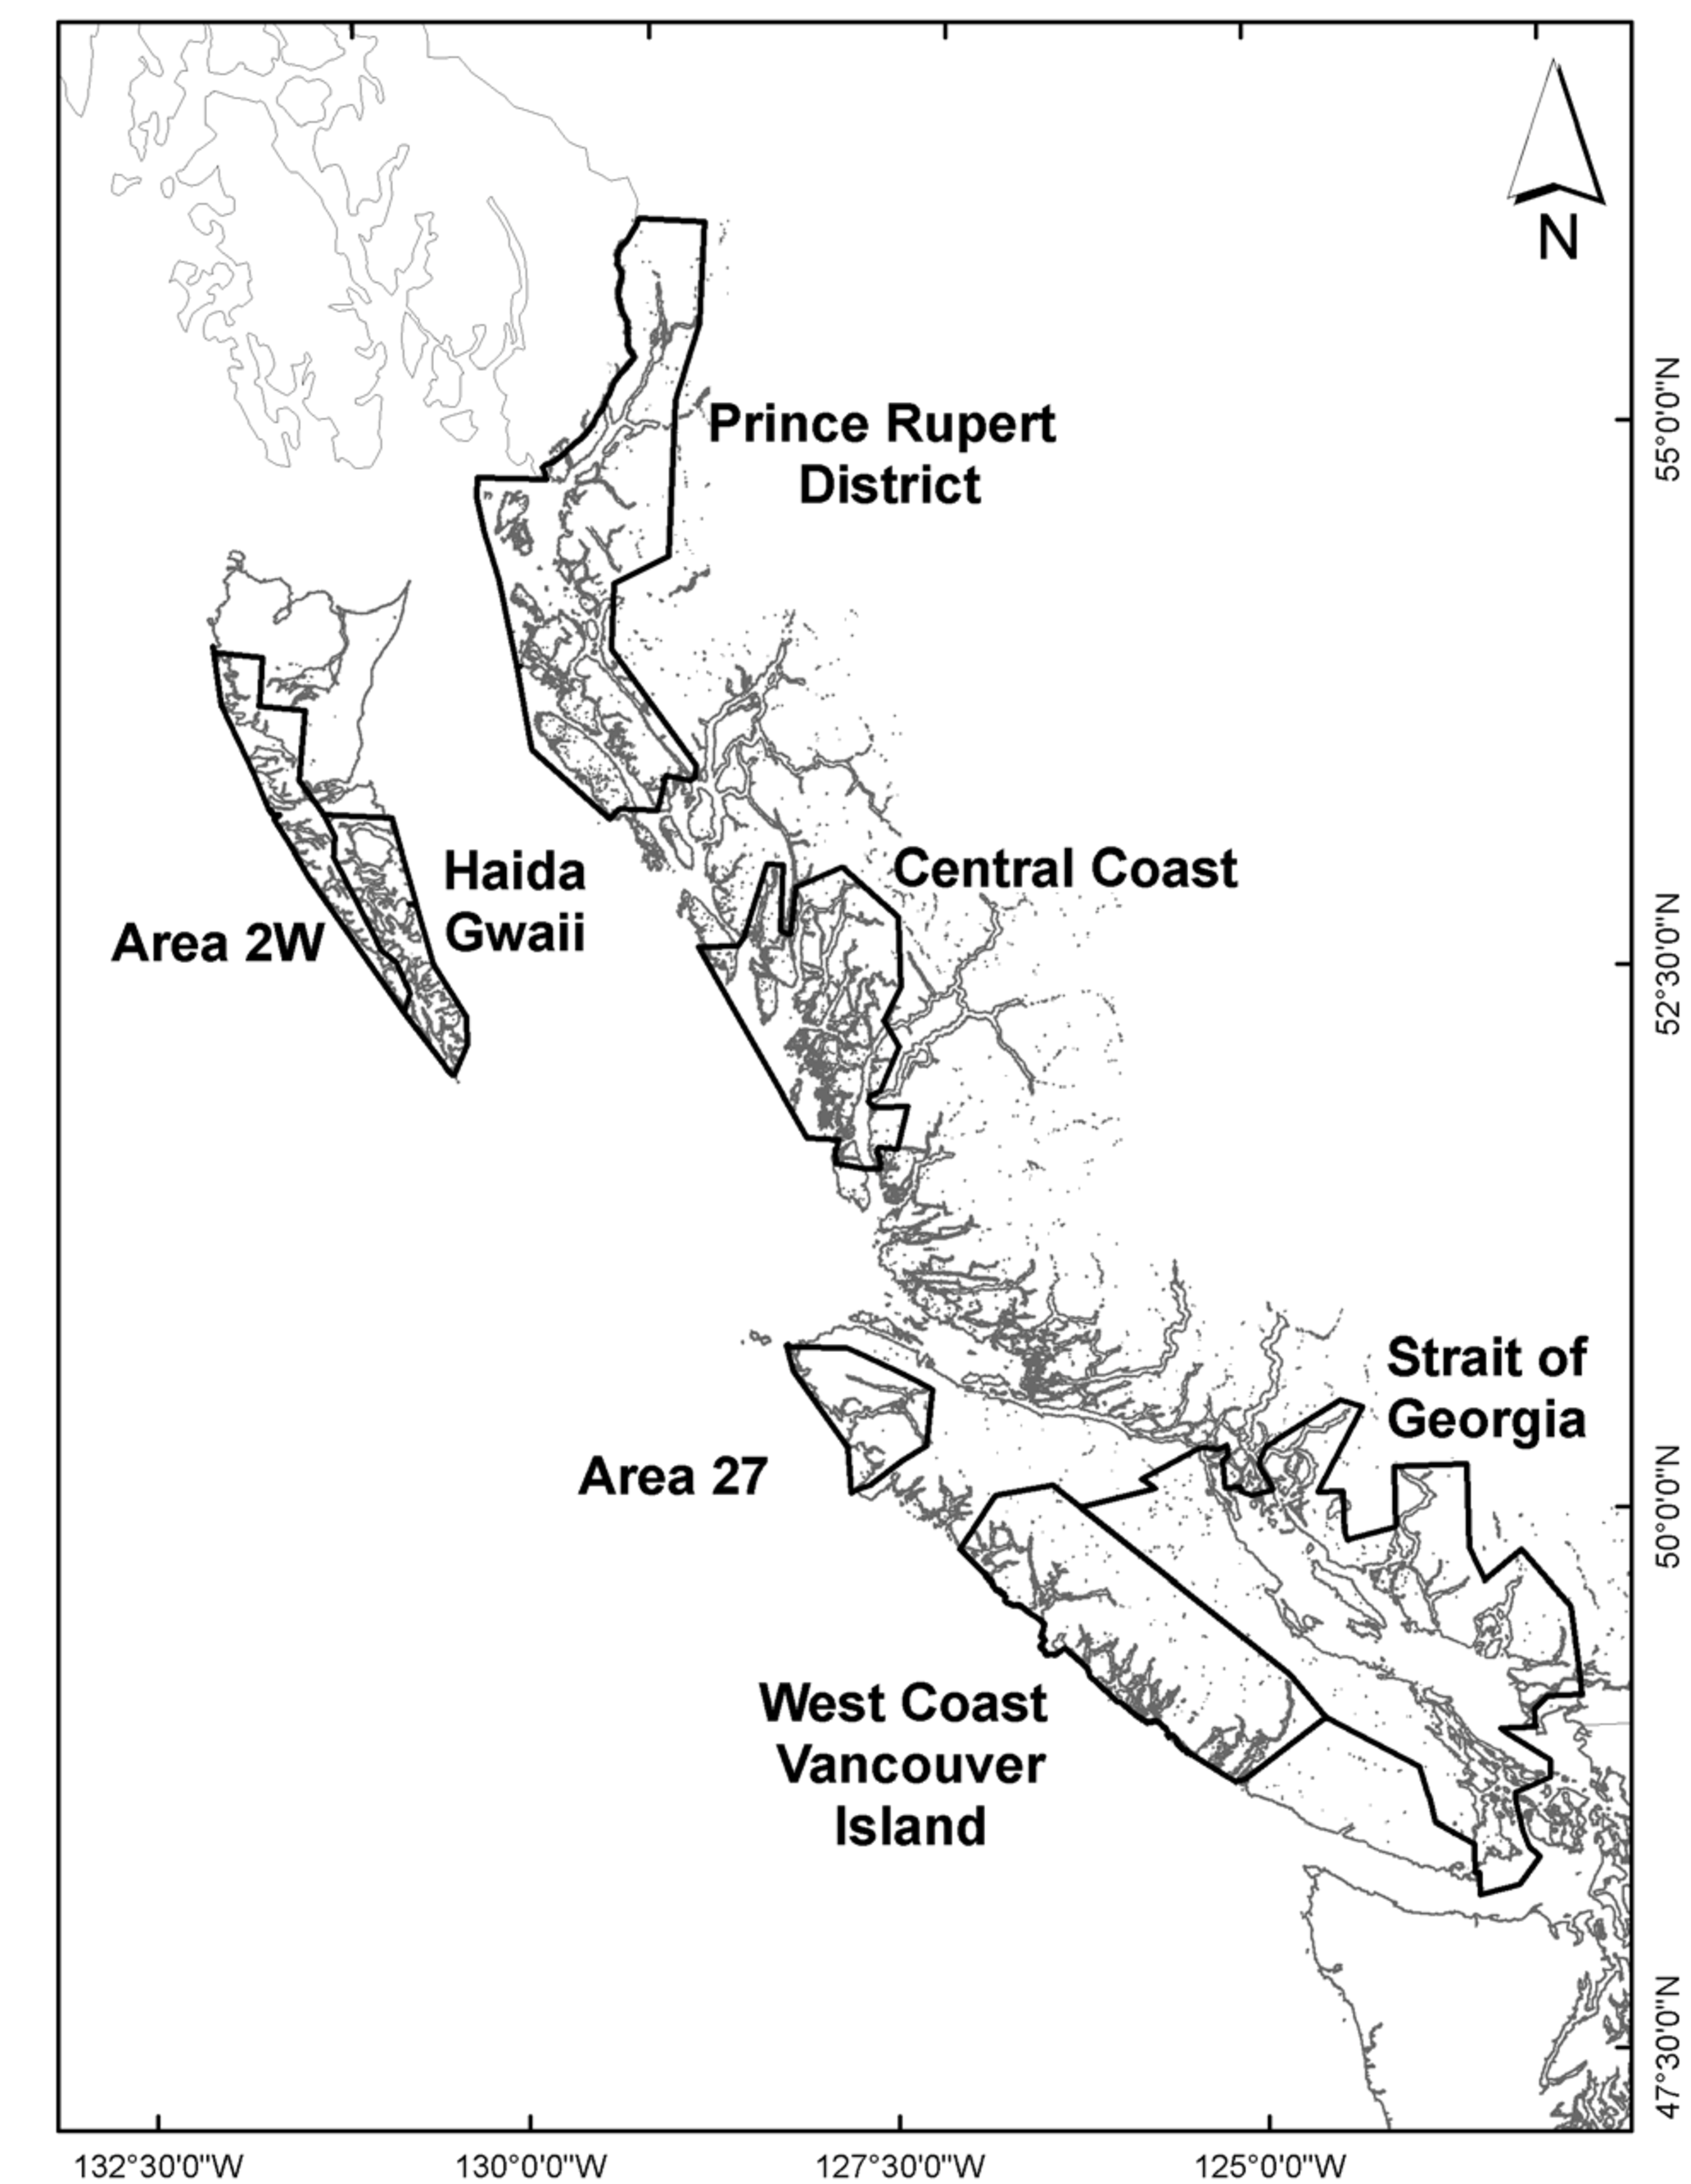
\includegraphics[width=\textwidth]{Figs/HerringAreaMap.pdf}
	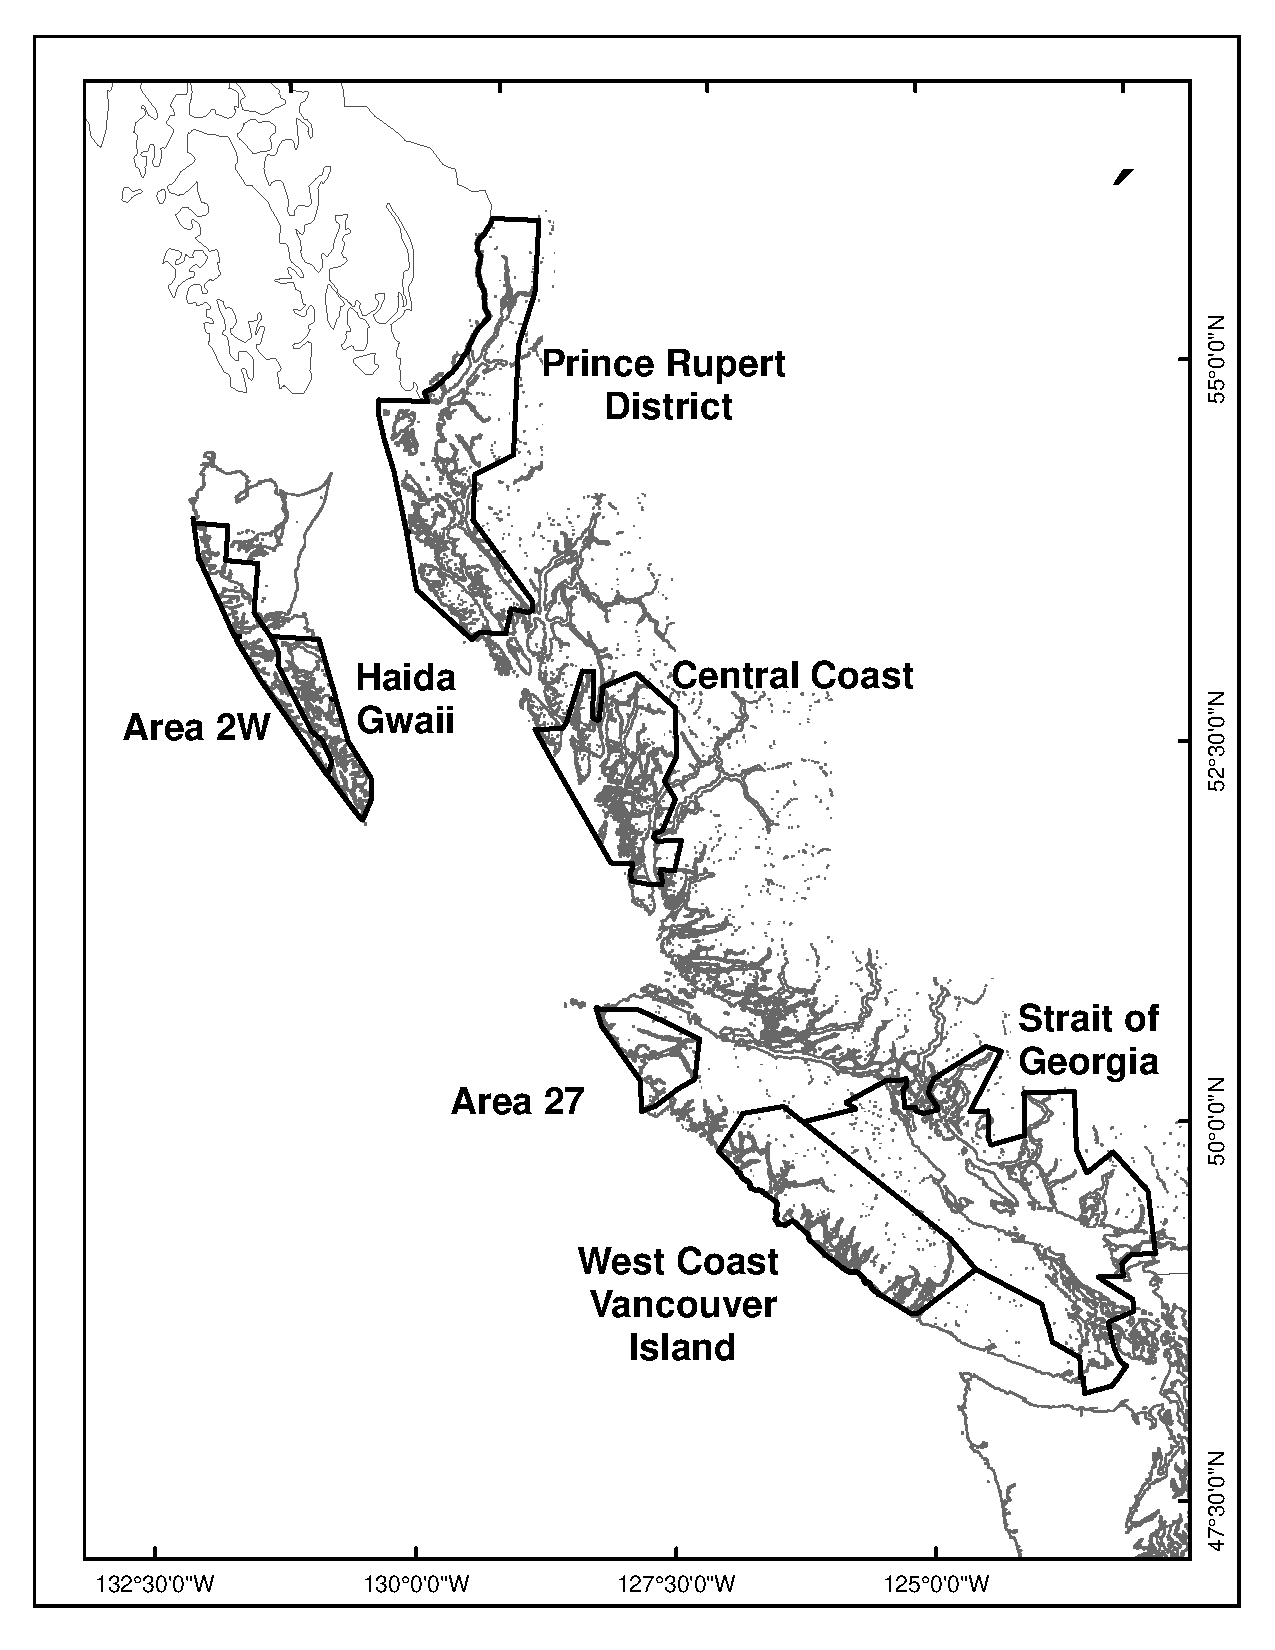
\includegraphics[width=\textwidth]{PBSfigs/Assessment_Regions_2W_27_2010_HG.pdf}
	\caption{B.C. herring major stock areas: Haida Gwaii (HG or QCI 2E), Prince Rupert District (PRD), Central
Coast (CC), Strait of Georgia (SOG), West Coast Vancouver Island (WCVI), and minor stock areas: Area 2W and
Area 27.}\label{Fig1}
\end{figure}
	
%%A reference for splines in selectivities can be found at \cite{aarts2009comprehensive}
%!TEX root = /Users/stevenmartell/Documents/CURRENT PROJECTS/iSCAM-trunk/fba/BC-herring-2011/WRITEUP/BCHerring2011.tex
\section{Methods}
	\subsection{Input data \& assumptions}
	\subsubsection{Catch data}
	For each of the statistical areas, the required input data for \iscam\ consists of a catch time series for each of the fishing fleets.  For the BC herring fishery, the annual total removals has been partitioned into three distinct fishing fleets (or fishing periods, see Figure \ref{FigCatch}).  The first fleet is a winter seine fishery that has been in operation since the start of the assessment in 1951, the second is a seine-roe fishery that commenced in 1972 in the Strait of Georgia, and the third fleet is a gillnet fishery that targets females on the spawning grounds. The model is fit to the catch time series information and assumes measurement errors are lognormal, independent and identically distributed.  The assumed standard deviation in the catch observations must be specified in the control file and it is assumed that measurement errors in the catch is the same for all fishing periods.  The units of the catch are given in 1000s of metric tons.
	
	In addition to the commercial catch, removals from fisheries independent surveys must also be specified in \iscam. Two additional fleets are specified to represent the spawn survey, where the spawn survey is broken into two distinct time periods pre-1988 and post-1988, the year when the survey switched from surface surveys to dive surveys.  This partitioning of the data is done for two reasons: (1) to allow for different catchability coefficients to be specified for the early and late periods, and to allow for more weight to be placed on the contemporary data due to improved precision in the estimates of egg layers. 

%TODO decide if the test fishery data is going to be looked at here or in the appendix
	In the case where the test fishery data has been separated from the seine roe fishery, an additional fleet is specified in the data file and fishing mortality rates for the test fishery are also estimated in years when the catch is greater than 0.
	
\begin{figure}[!tbp]
	% Requires \usepackage{graphicx}
	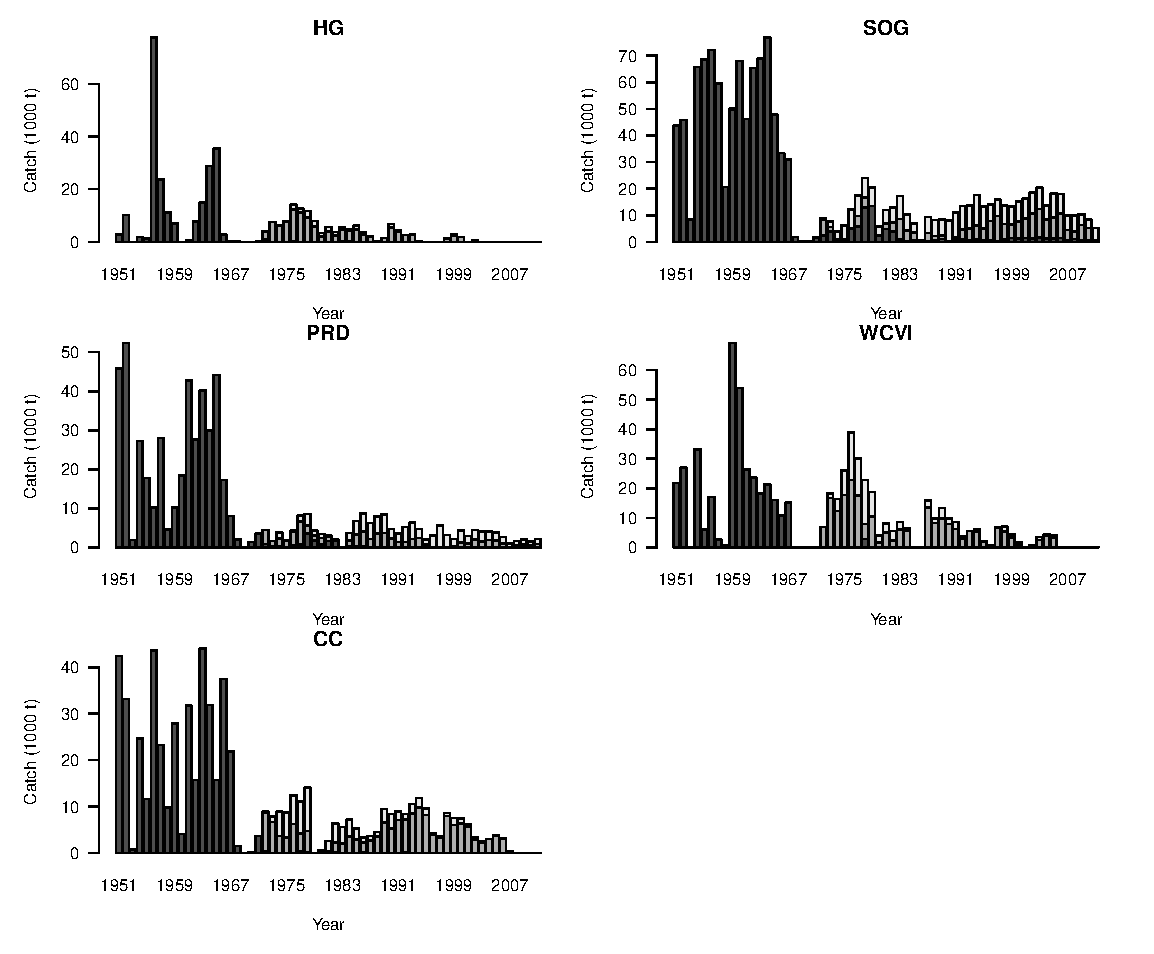
\includegraphics[width=\textwidth]{../Figs/iscam_fig_CatchMajorAreas.pdf}\\
	\caption{Historical catch of herring in the five major stock areas between 1951 and 2011 for the winter purse seine fishery (dark bars), seine-roe fishery (grey bars), and gillnet fishery (light grey bars). Units of catch are in thousands of metric tons.}\label{FigCatch}
\end{figure}
	
	\subsubsection{Relative abundance data}
Herring spawn surveys have been conducted throughout the B.C. coast beginning in the 1930s. Prior to 1988, spawn surveys were conducted from the surface either by walking the beach at low tide or using a drag from a skiff to estimate the shoreline length and width of spawn. Egg layers were sampled visually and are used to calculate egg densities following the methods of \cite{schweigert2001stock}. Beginning in 1988, herring spawn surveys using SCUBA methods were introduced and were implemented coastwide within a couple of years initially being conducted by DFO staff and eventually through contract divers hired through the test fishing program. Prior to the 2006 Larocque ruling, the test fishing program was funded through an allocation of fish by industry. In years since the 2006 Larocque ruling, the availability of resources to conduct dive surveys in all areas has been reduced. For 2011, dive surveys were conducted in all major and minor assessment regions, with the exception of Area 2W where snorkelling and surface survey methods were also used. As in earlier years, a few minor spawning beds outside the main assessment areas were surveyed by SCUBA or surface methods where resources permitted.


The locations of the spawning beds for the five major and two minor stock areas are shown in Figure \ref{figSpawnMaps}.  Egg density estimates are used to calculate a fishery-independent index of herring spawning biomass, referred to as the spawn survey index hereafter \citep{schweigert2001stock}.

\begin{figure}[!tbp]
	% Requires \usepackage{graphicx}
	\centering
	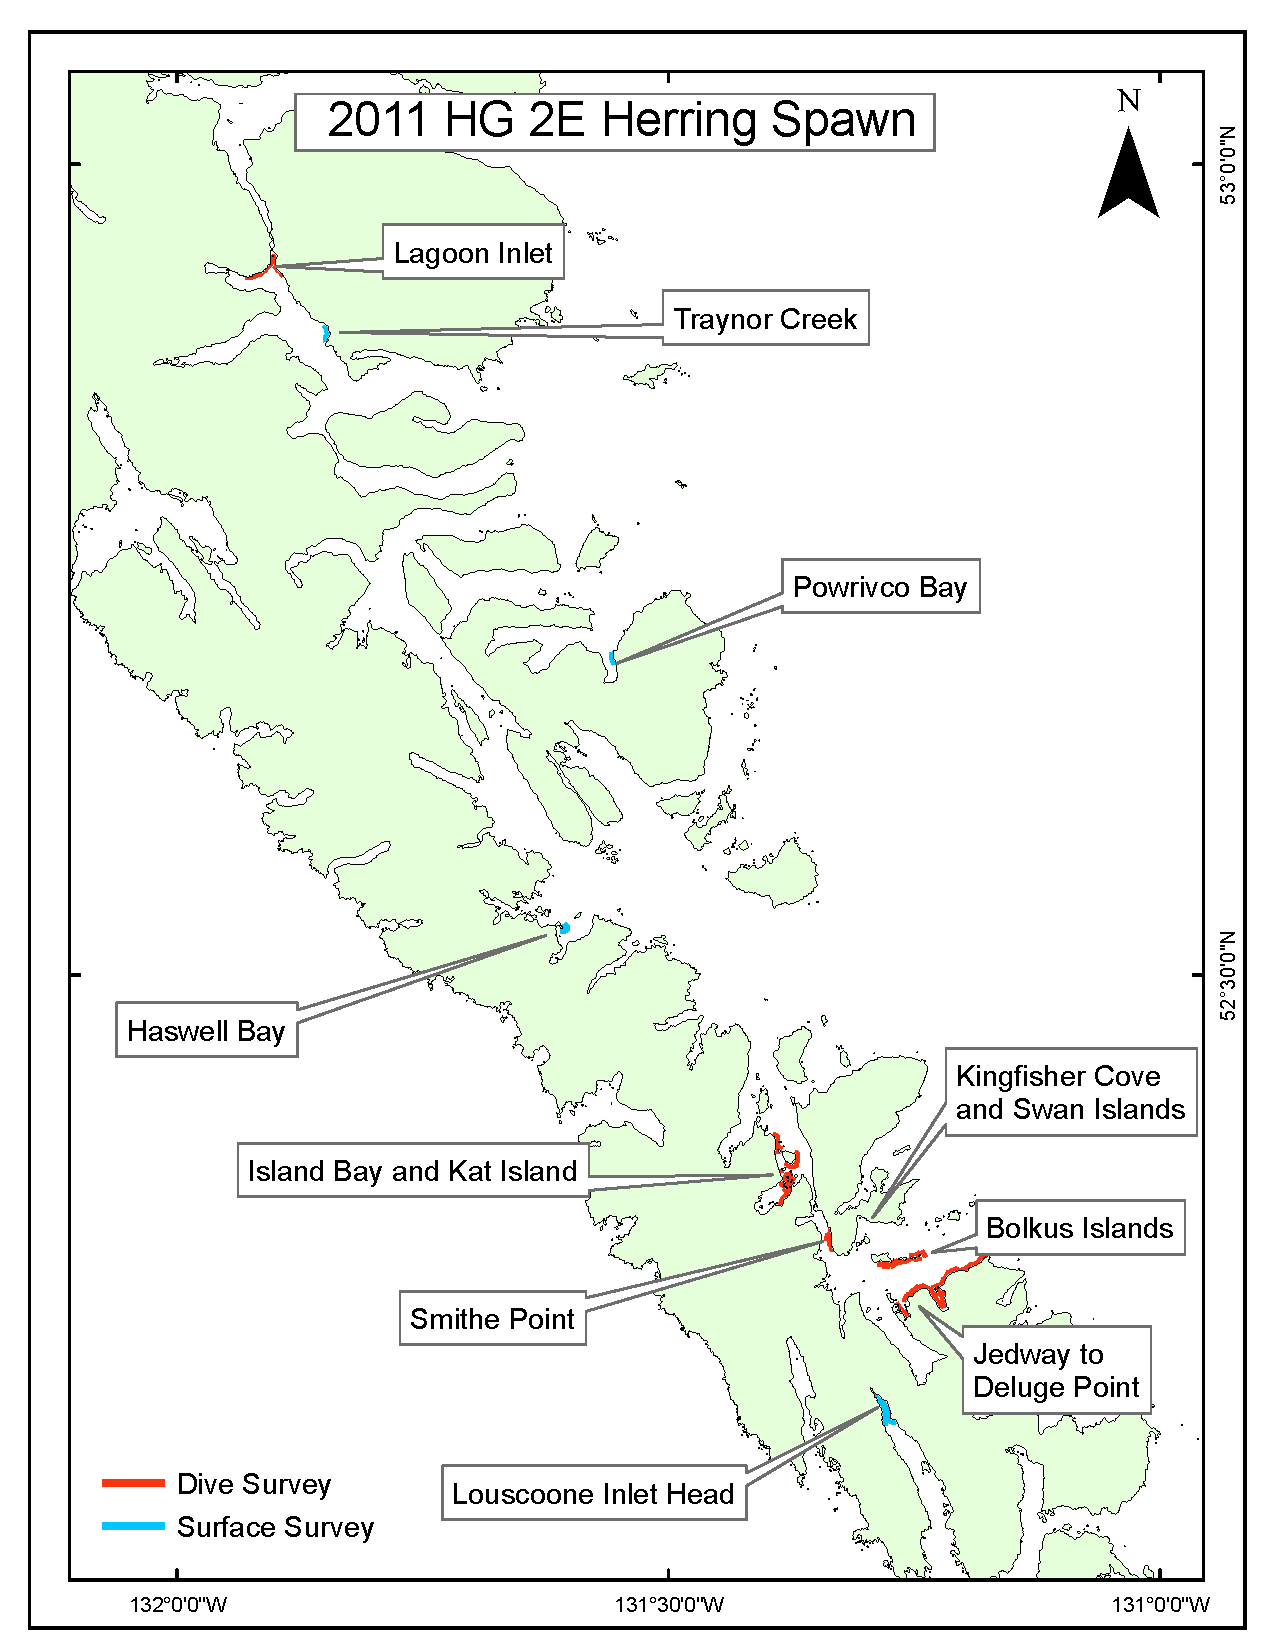
\includegraphics[scale=0.35]{../Figs/PBSfigs/2011_spawn_HG_2E_July13.pdf}
	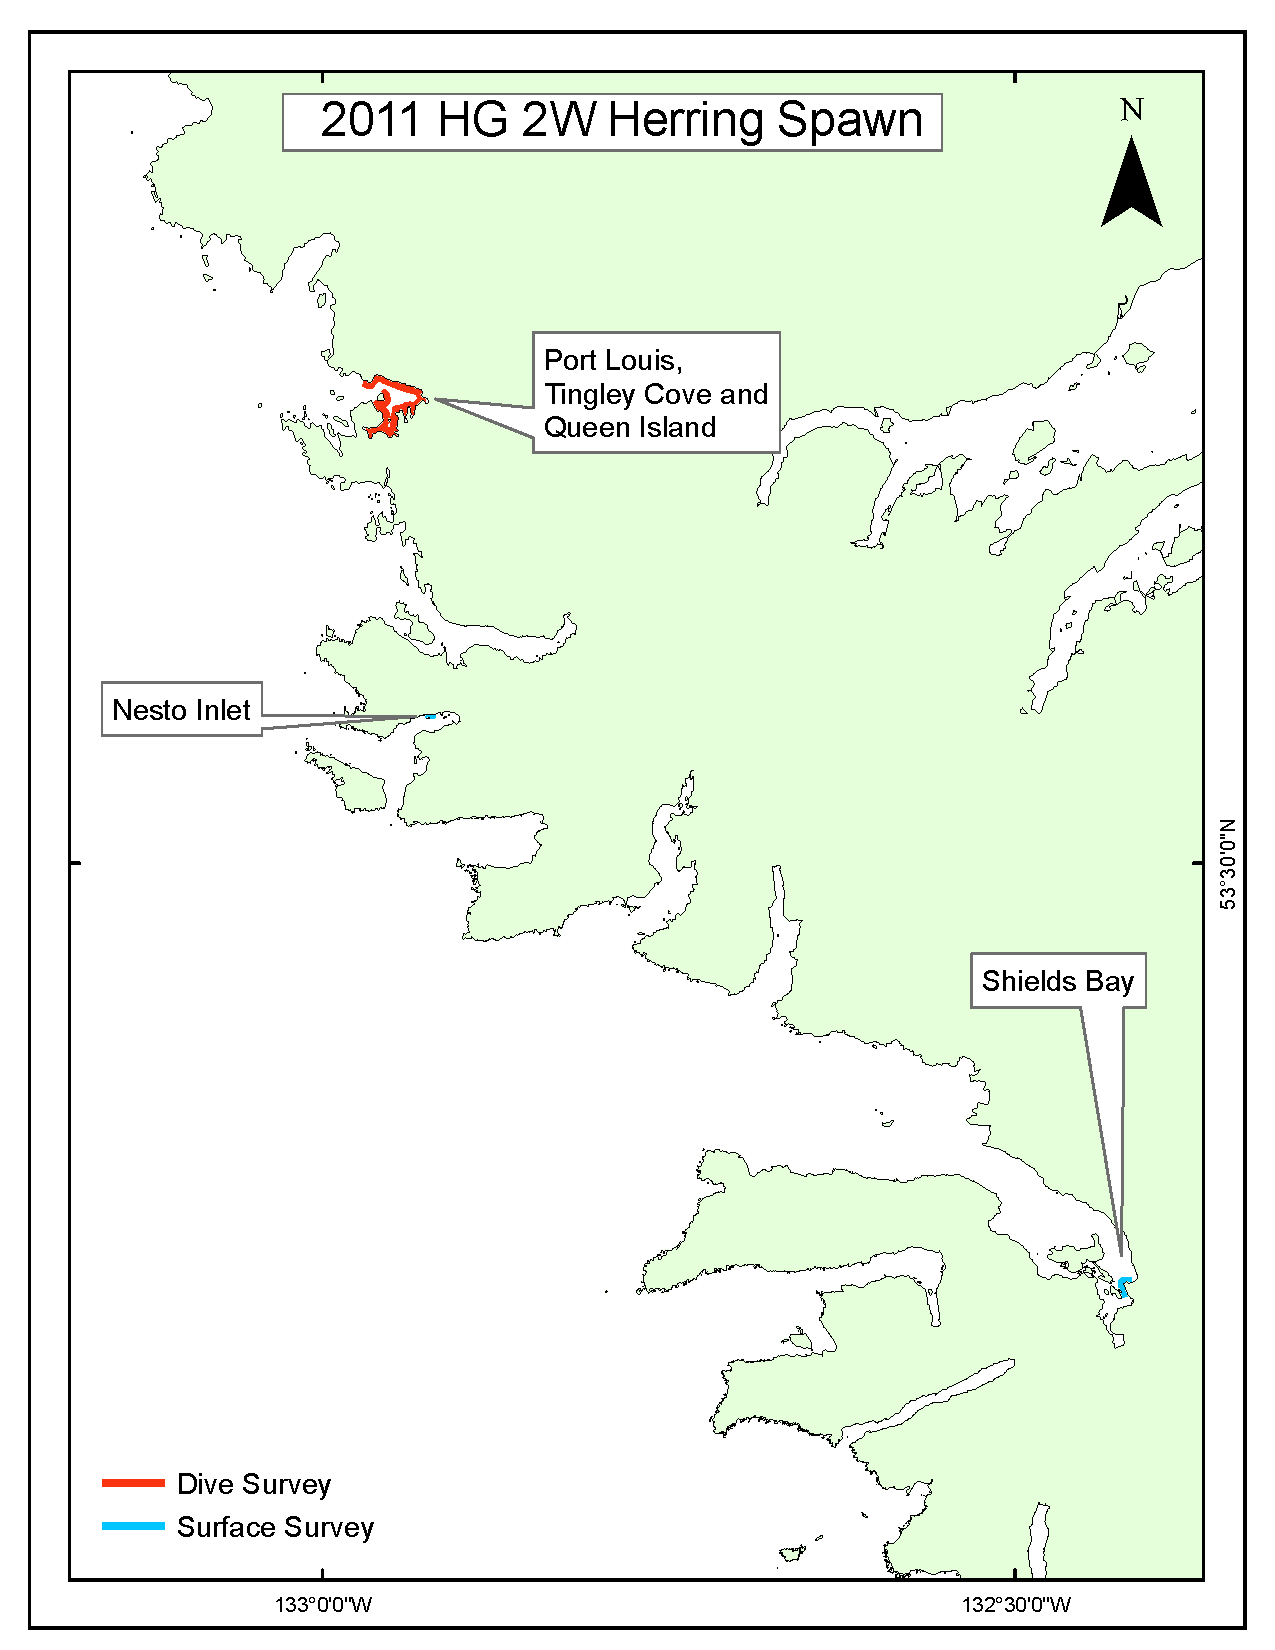
\includegraphics[scale=0.35]{../Figs/PBSfigs/2011_spawn_HG_2W_July13.pdf}\\
	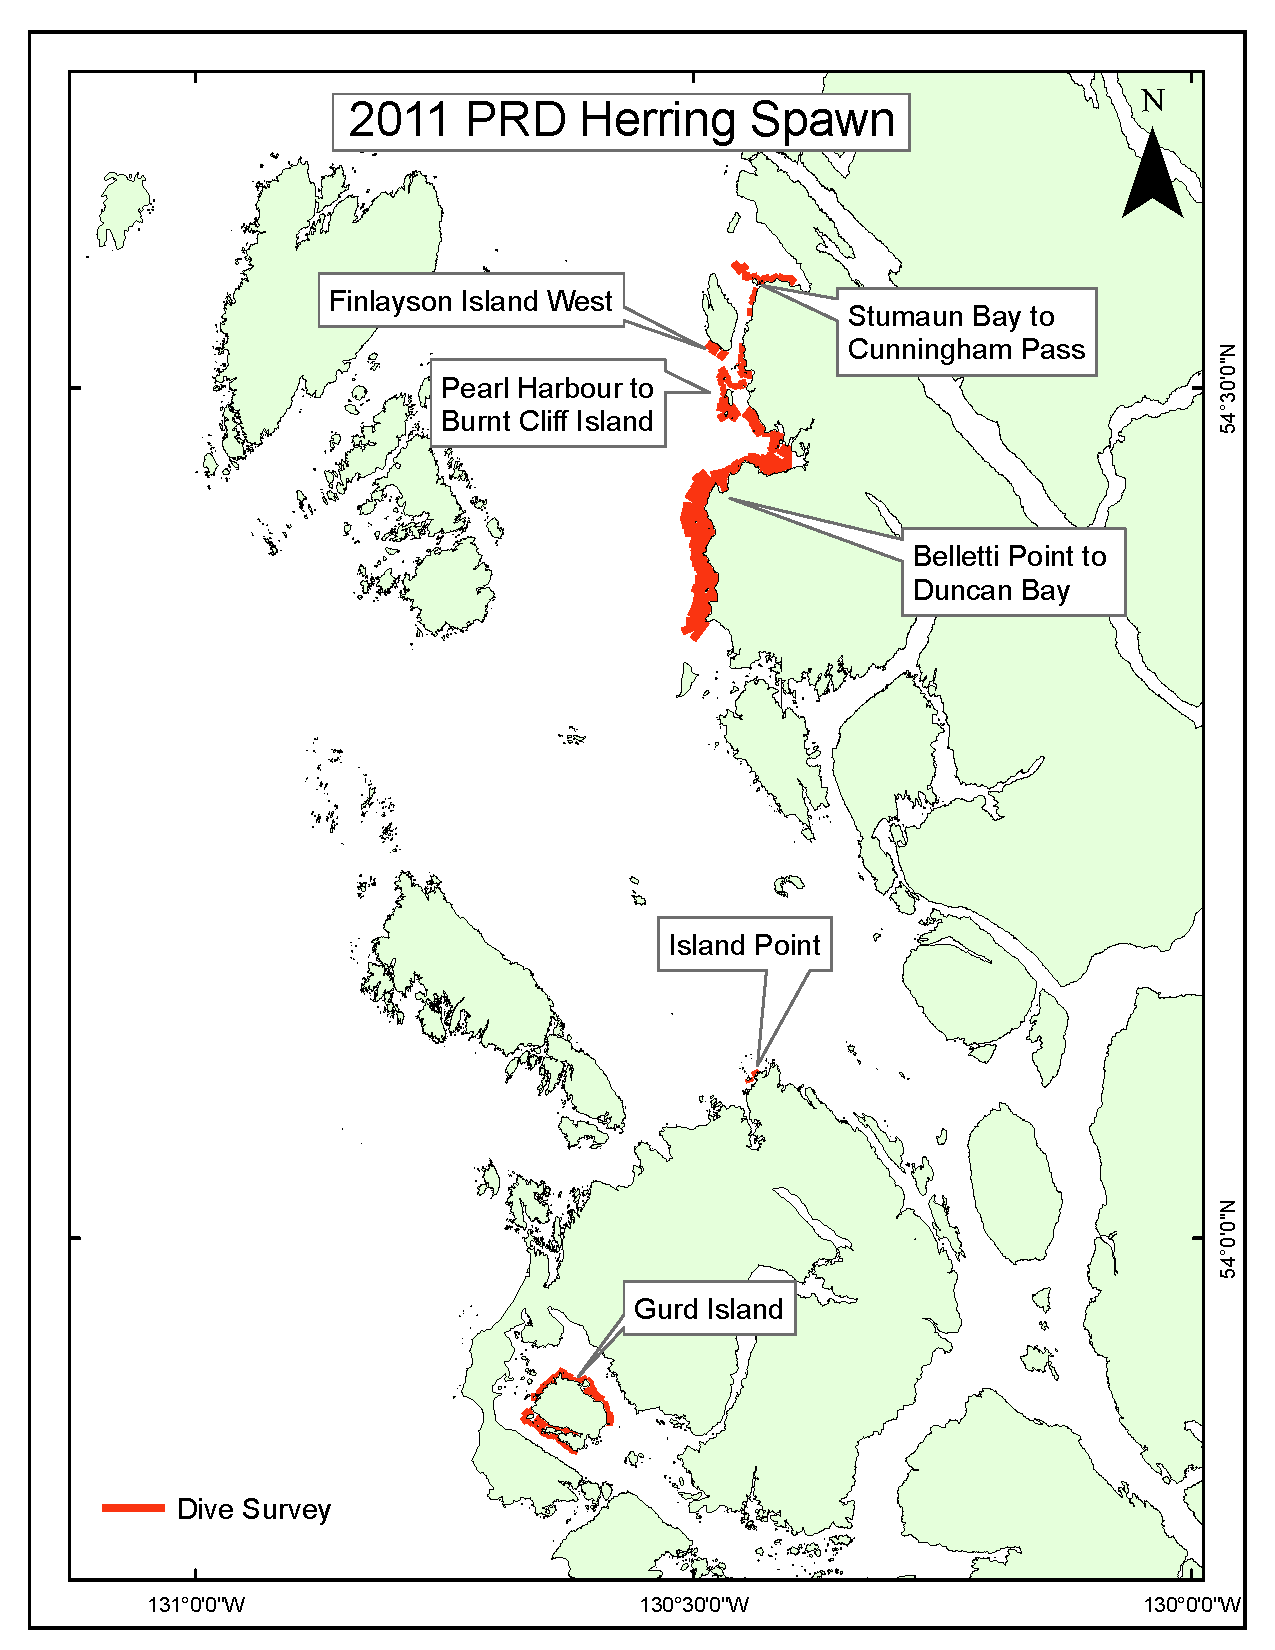
\includegraphics[scale=0.35]{../Figs/PBSfigs/2011_spawn_PRD_July13.pdf}
	\caption{Preliminary Spawning activity for Haida Gwaii (top panels) and Prince Rupert District (bottom) in 2011.}
\end{figure}
\begin{figure}[!tbp]
	% Requires \usepackage{graphicx}
	\ContinuedFloat
	\centering
	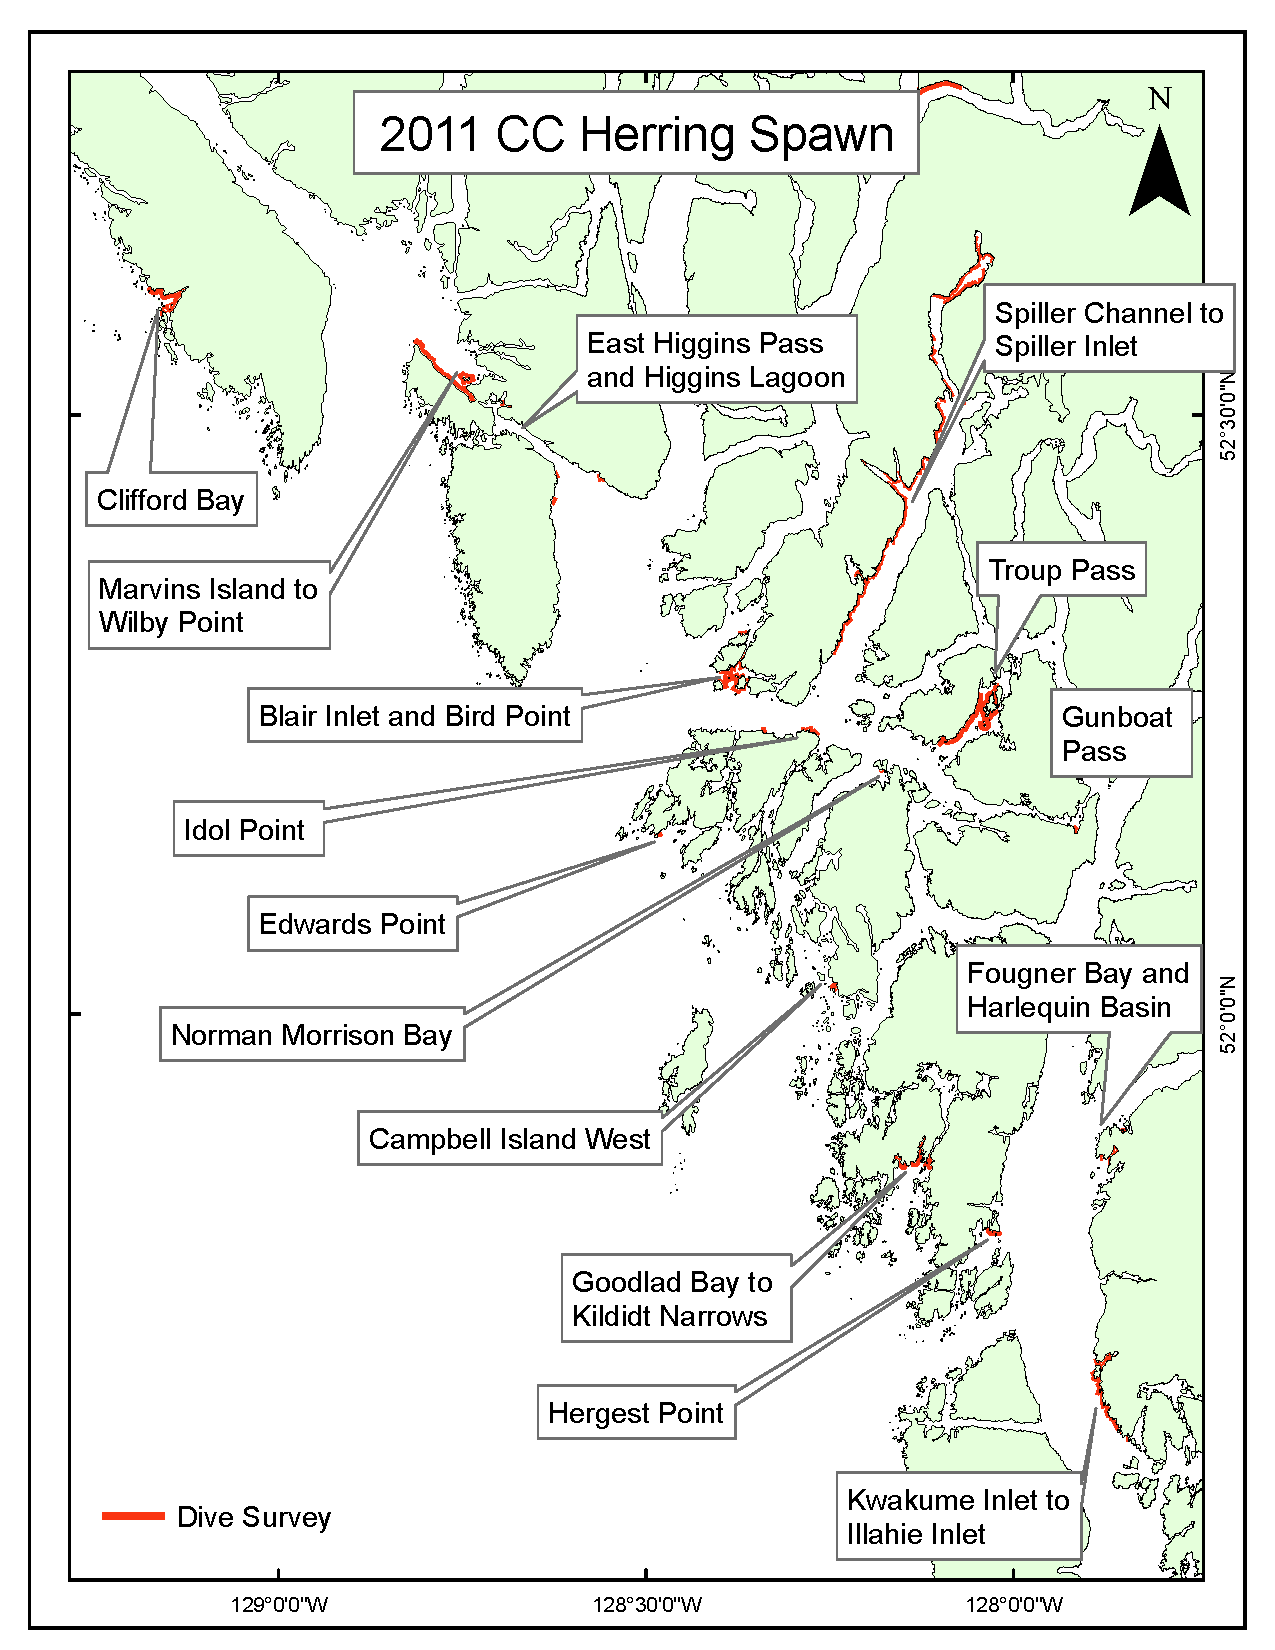
\includegraphics[scale=0.35]{../Figs/PBSfigs/2011_spawn_CCJuly13.pdf}
	%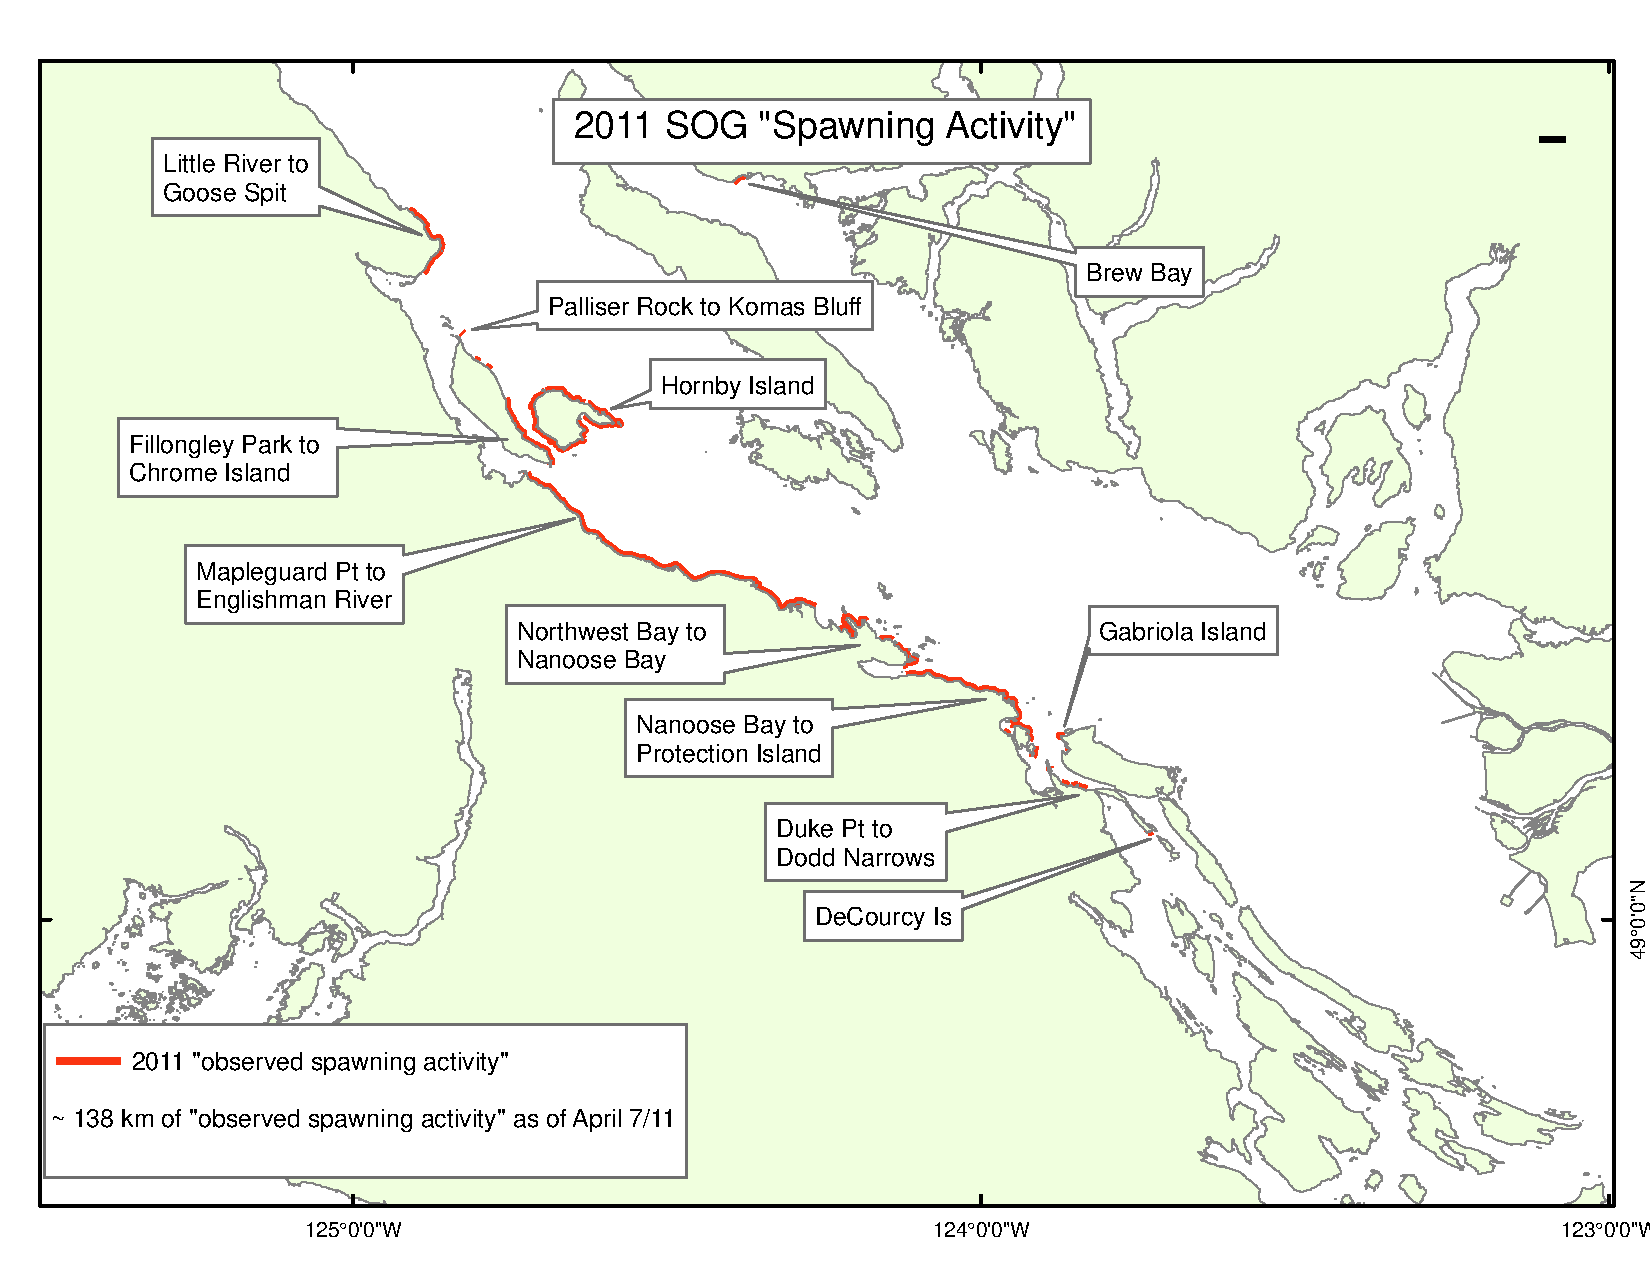
\includegraphics[scale=0.5]{../Figs/PBSfigs/2011-SOG-Prelim-WG.pdf}
	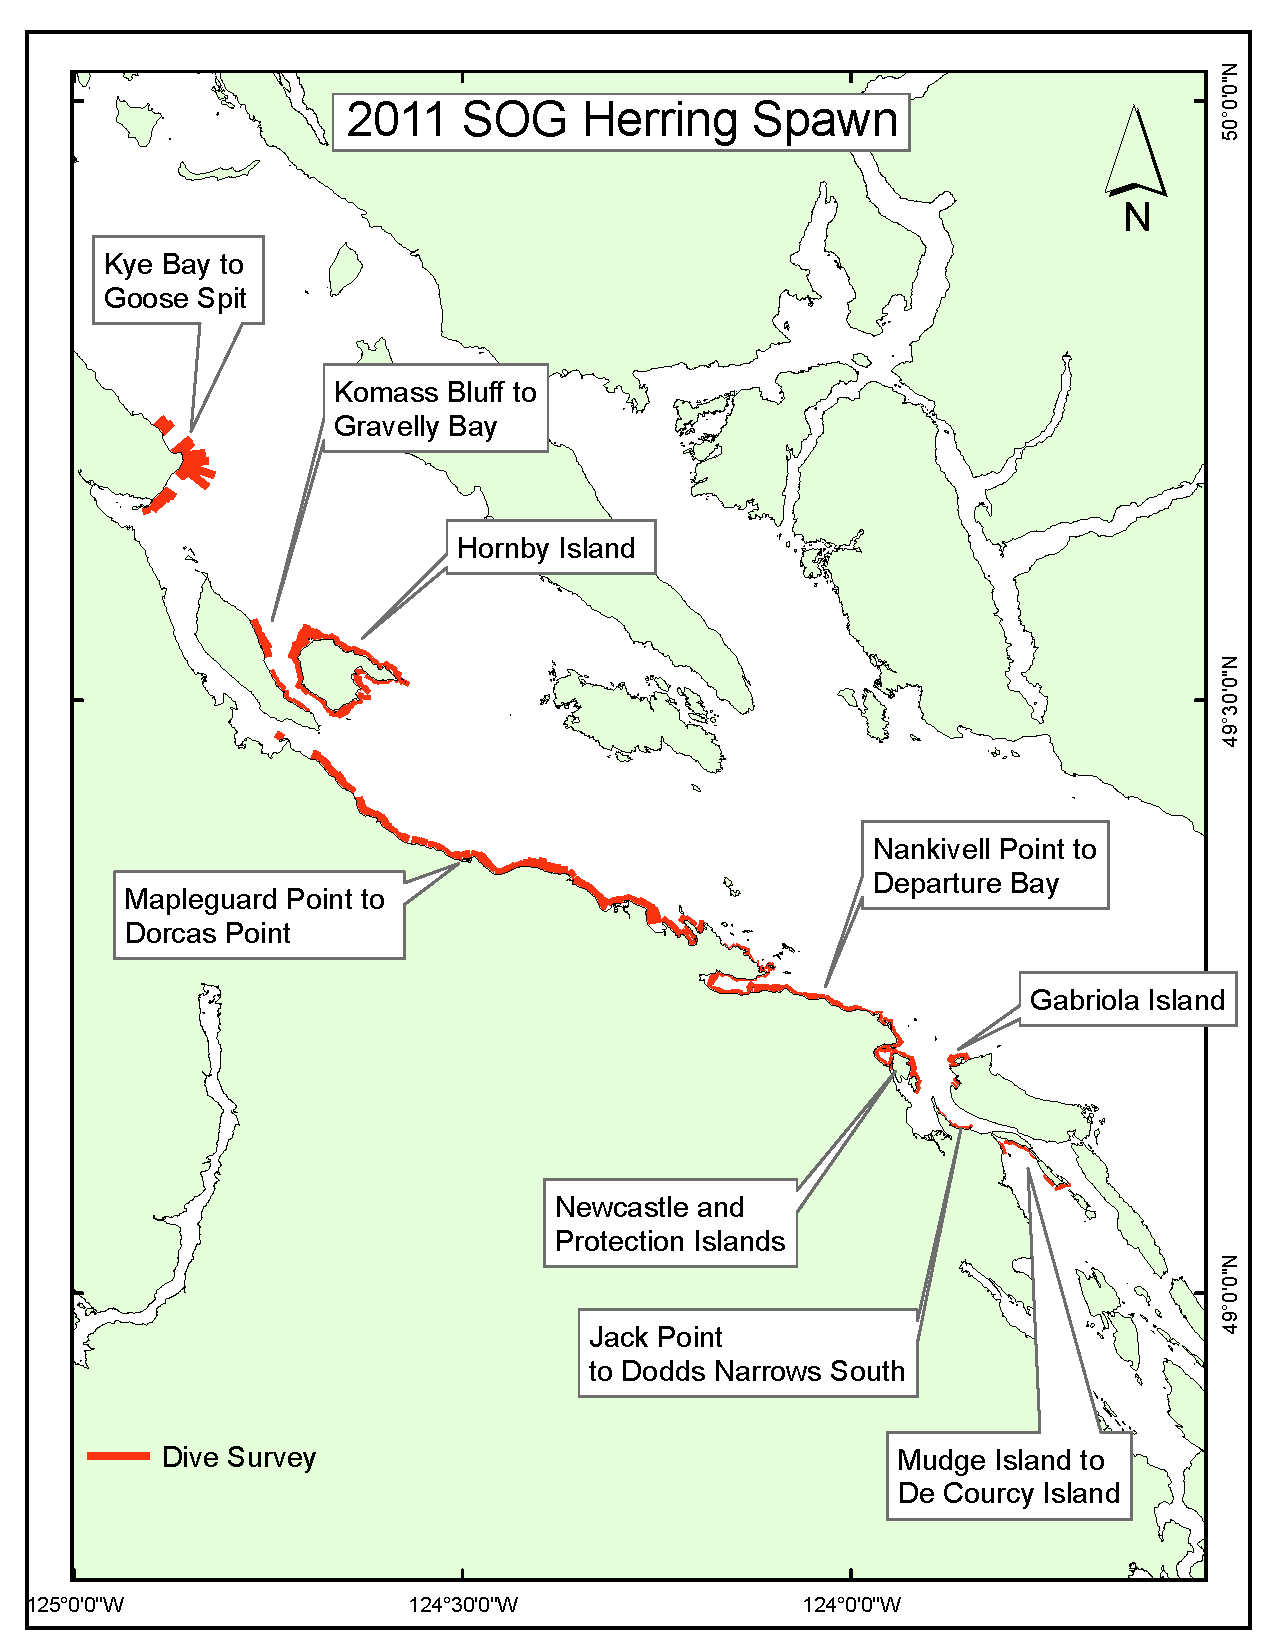
\includegraphics[scale=0.35]{../Figs/PBSfigs/2011_spawn_SOG_July13.pdf}\\
	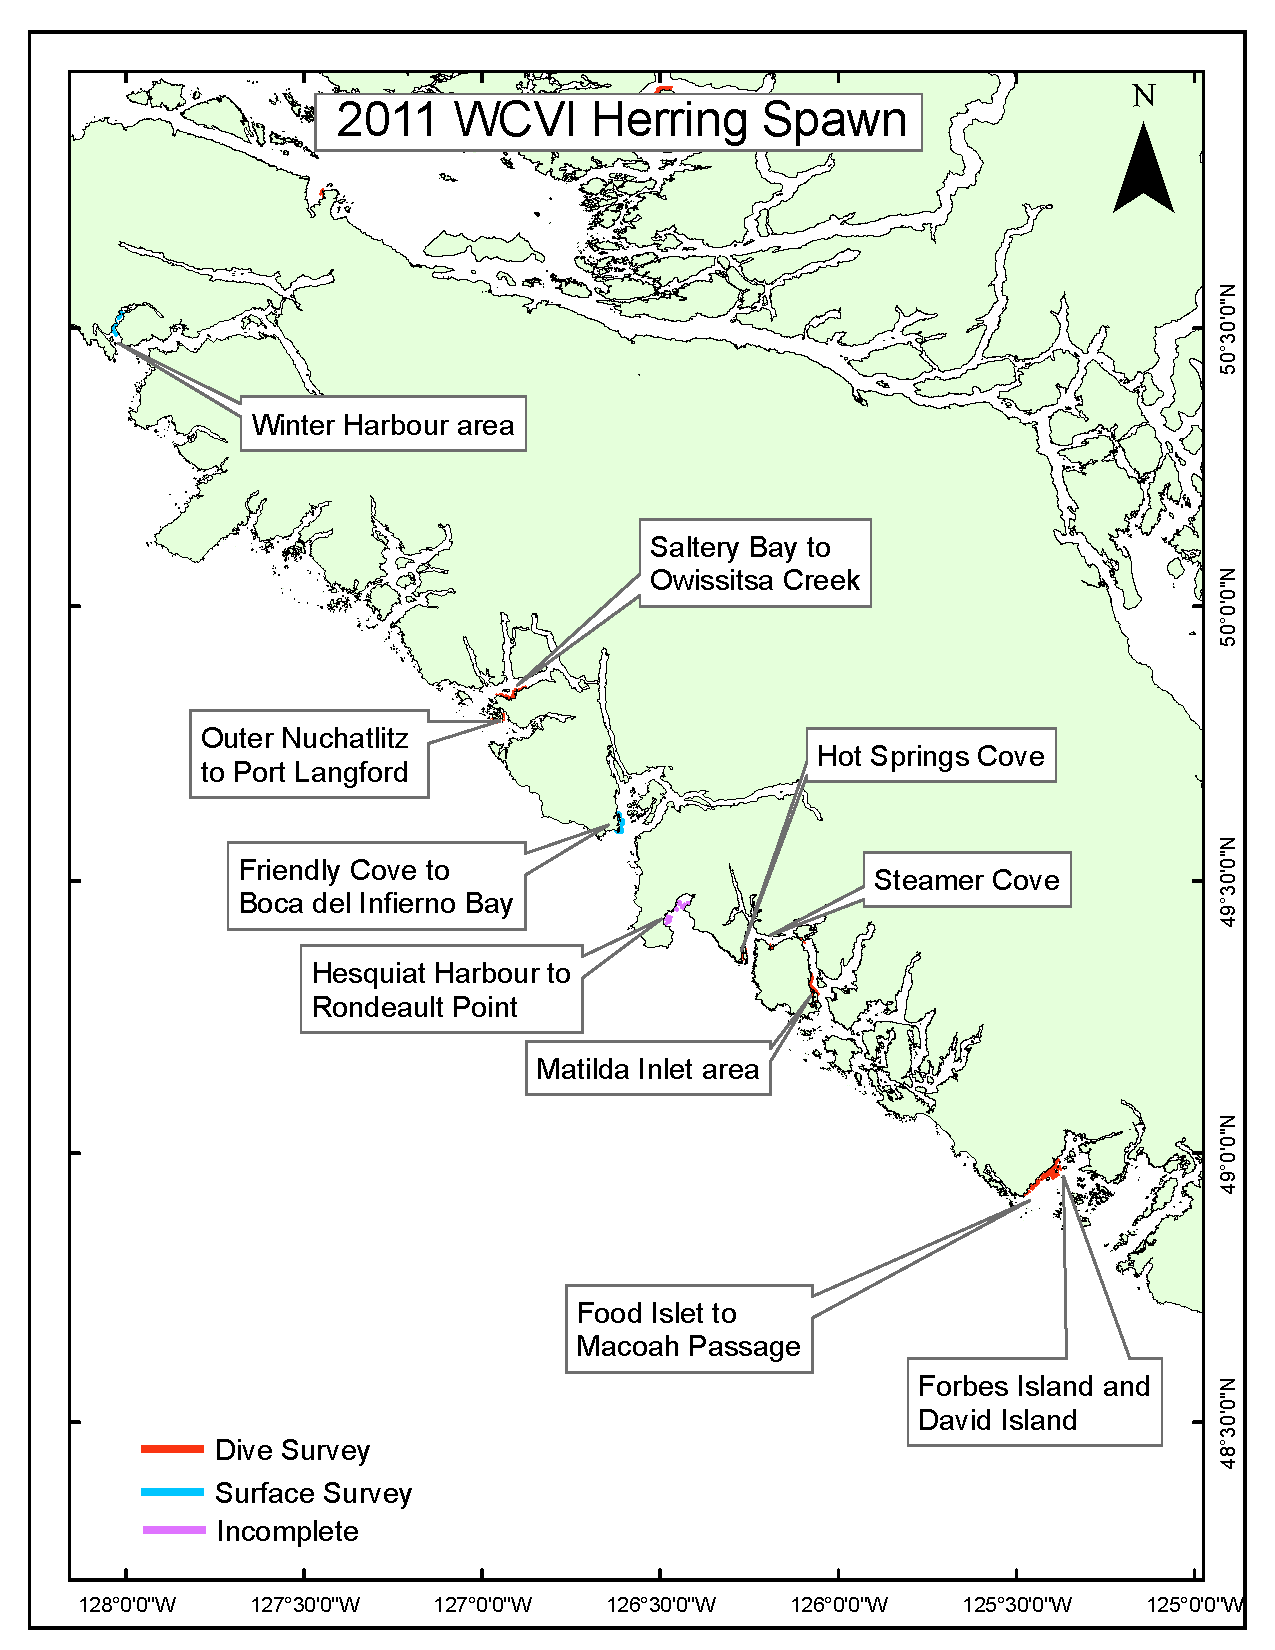
\includegraphics[scale=0.35]{../Figs/PBSfigs/2011_spawn_WCVI_August16.pdf}
	\caption{Preliminary Spawning activity for Central Coast (top left panel), Strait of Georgia (top right) in 2011 and west coast Vancouver Island (bottom).}\label{figSpawnMaps}
\end{figure}
% \begin{figure}[!tbp]
% 	% Requires \usepackage{graphicx}
% 	\ContinuedFloat
% 	\centering
% 	%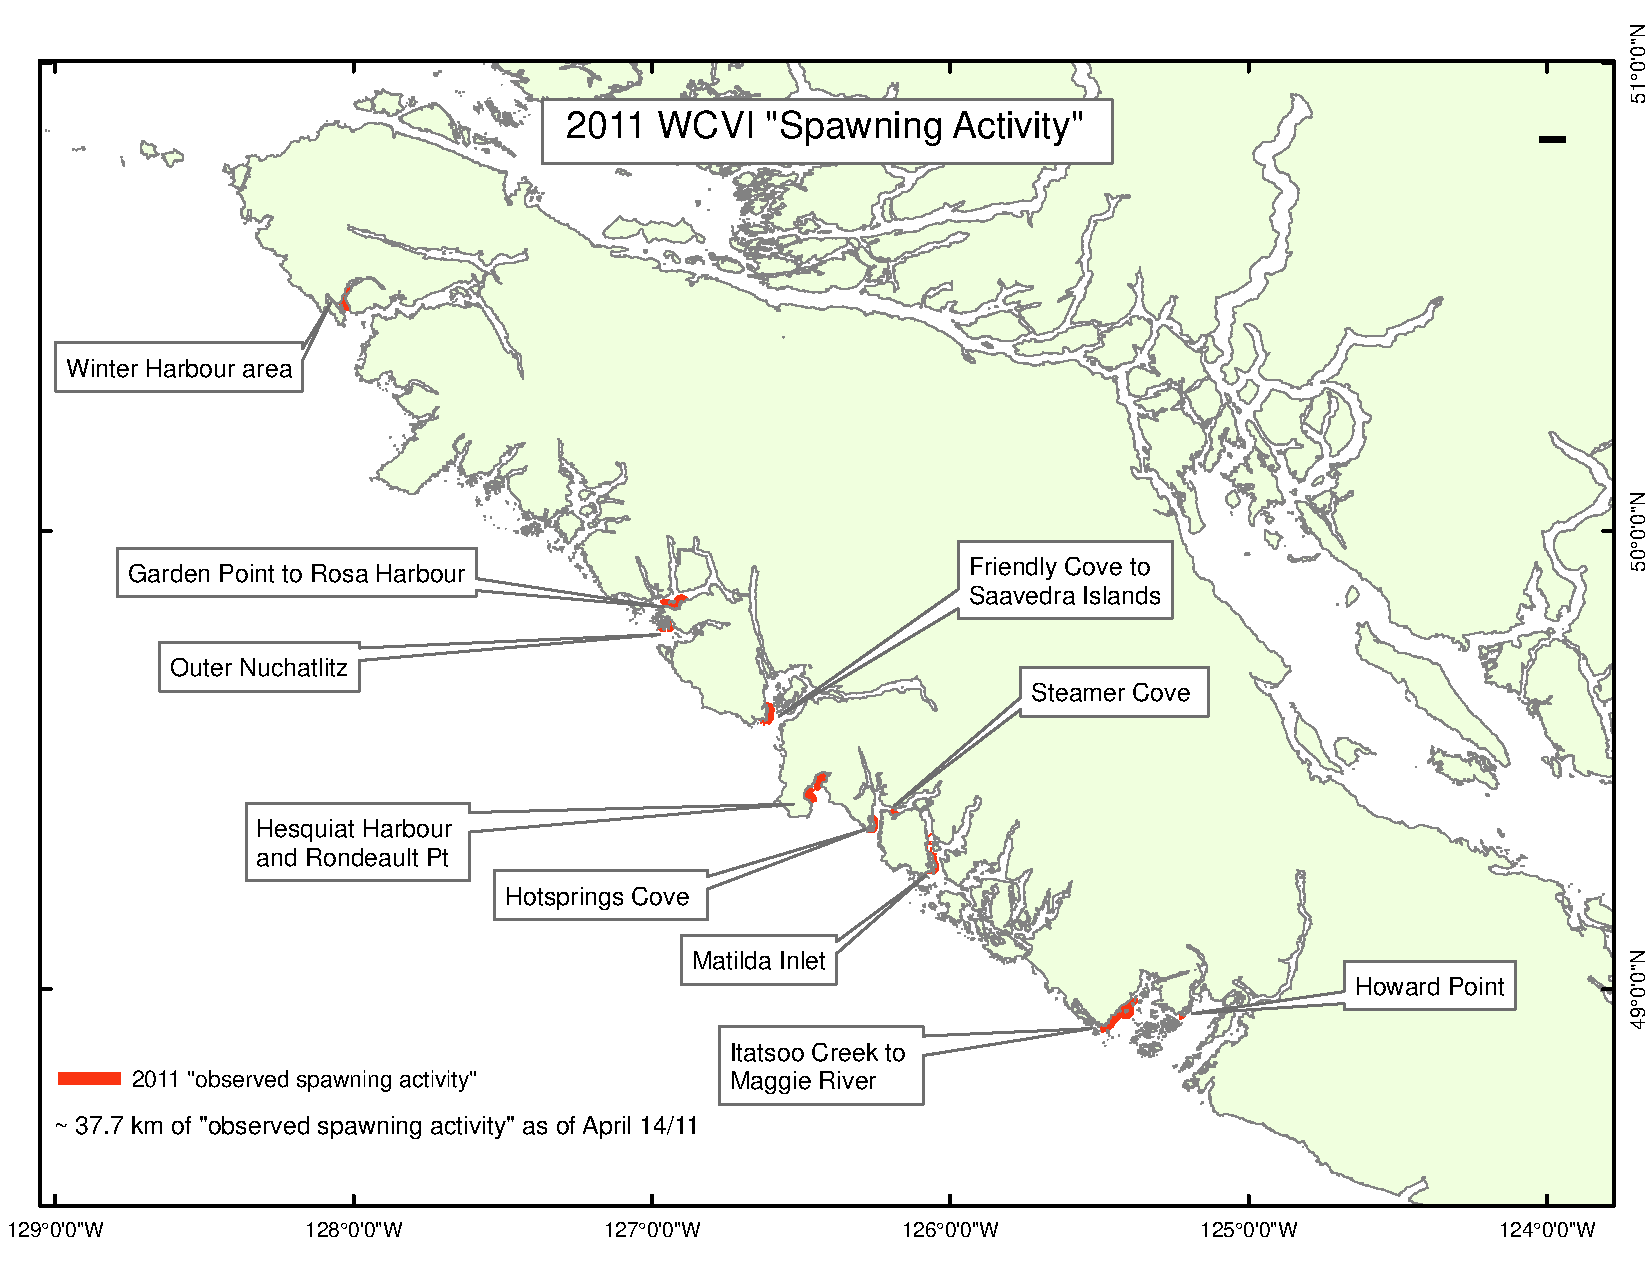
\includegraphics[scale=0.5]{../Figs/PBSfigs/2011-WCVI-Prelim-WG.pdf}\\
% 	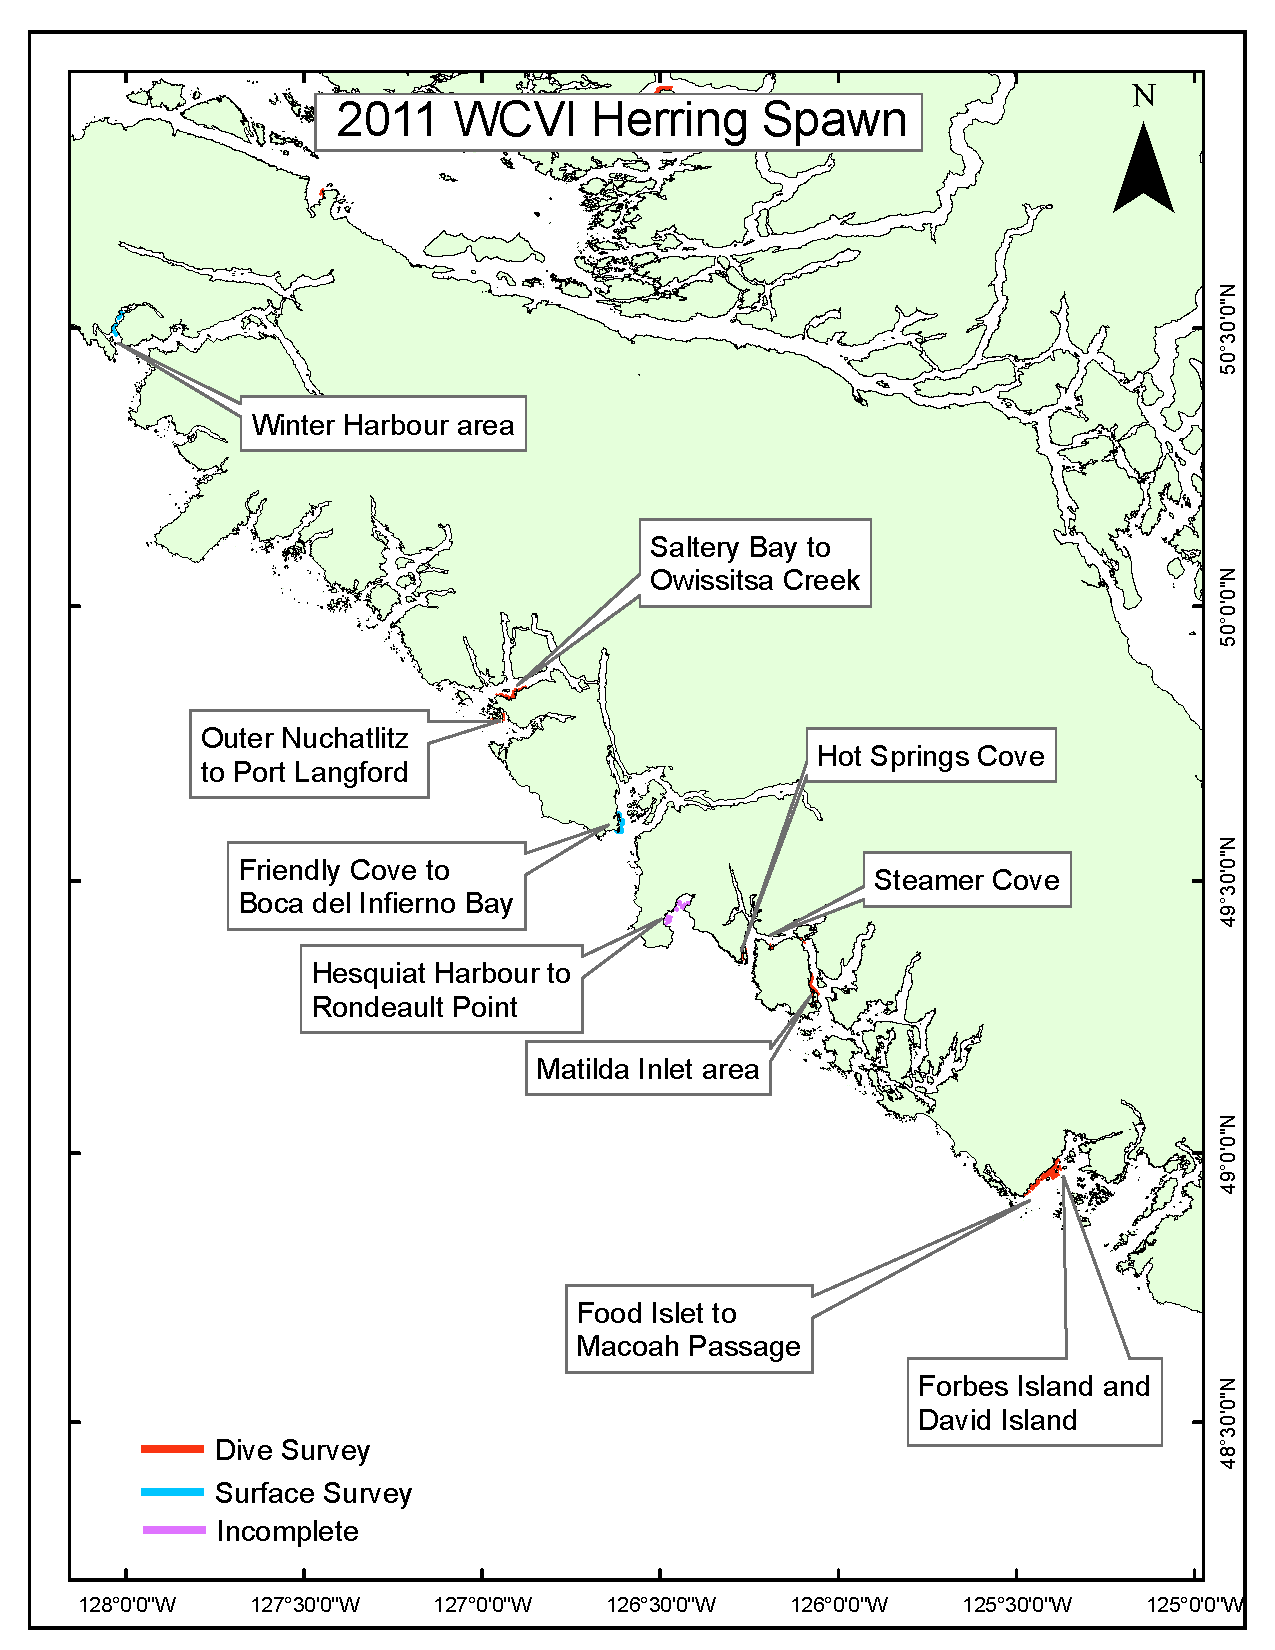
\includegraphics[scale=0.5]{../Figs/PBSfigs/2011_spawn_WCVI_August16.pdf}\\
% 	\caption{Preliminary Spawning activity in 2011 for the West Coast of Vancouver Island (includes minor stock area 27).}\label{figSpawnMaps}
% \end{figure}

	The spawn survey is conducted after the fisheries in the area have been completed; therefore, it is assumed that all the mortality for the year has occurred just prior to commencing the spawning survey. The fisheries independent survey estimates egg density and total spawn area, and from this information the total female spawning biomass can be estimated assuming the 200 eggs per gram of female  or 100 eggs per gram of mature  individuals \citep{hay1985reproductive,hardwick1973biomass}. The assumed selectivity for the spawn survey is fixed to the maturity schedule for herring.  	
	
\begin{figure}[!tbp]
	% Requires \usepackage{graphicx}
	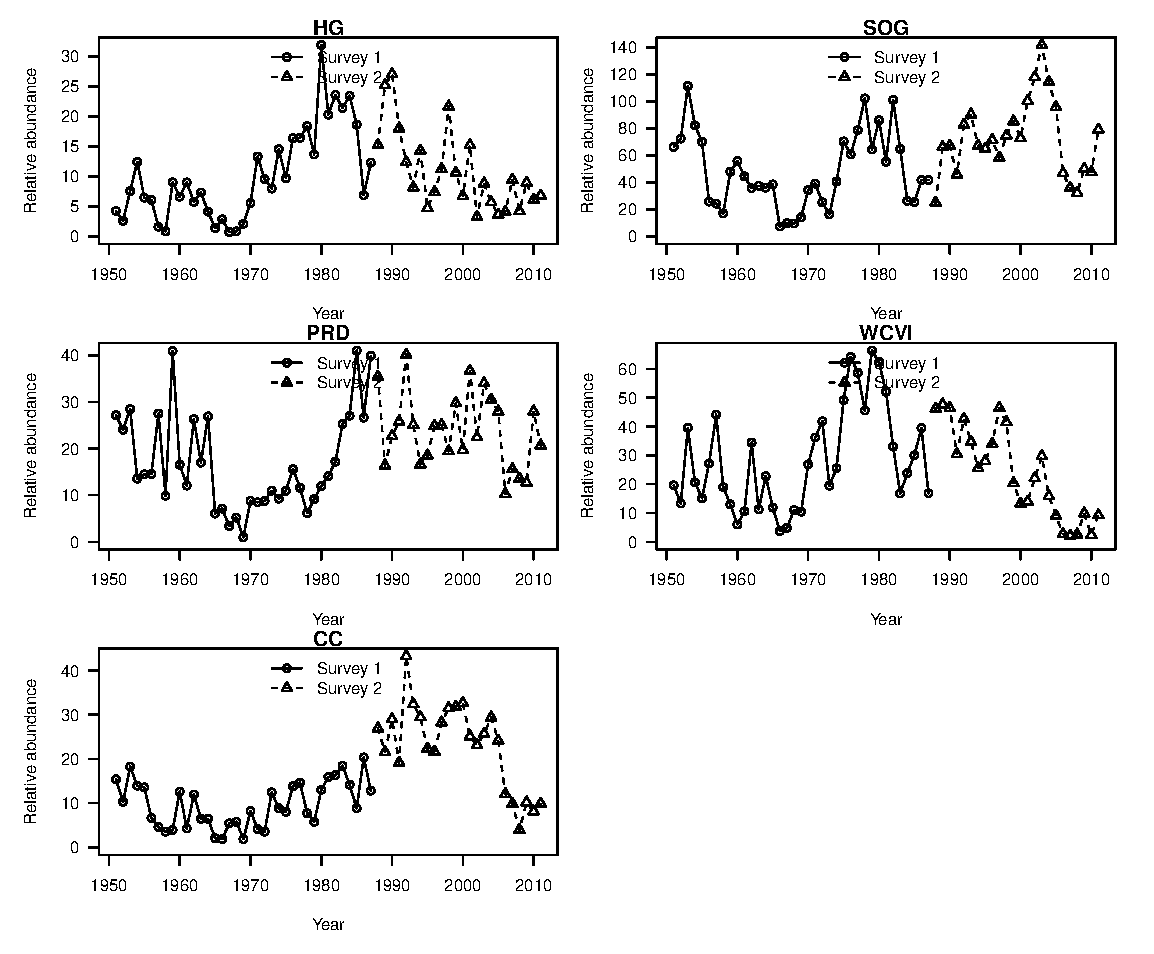
\includegraphics[width=\textwidth]{../Figs/iscam_fig_SurveyMajorAreas.pdf}\\
	\caption{Spawn survey index for Strait of Georgia between 1951 and 2011. The units are actual estimates of spawning biomass (1000s tons), but only the trend information is used in the model fitting.}\label{FigSurvey}
\end{figure}
	
	\subsubsection{Biological samples}
	
	Biological samples are collected from both commercial catch and from the test fishery program.  Commencing  in 1975, test fishery charters supplemented biological samples in areas with poor sampling that was not representative of the stock in that area (i.e., fishing solely on spawning aggregations), or in closed areas. Prior to 2006, test fishing charters were funded through an allocation of fish to the test program; the program is now fully funded by DFO.  Through a contract with DFO, the Herring Conservation and Research Society (HCRS) sub-contracts a number of vessels to collect biological samples.  Industry also conducts pre-season test sets for roe-quality testing in open areas and supplementary biological samples are provided as part of this program.  The following data are collected for all biological samples: fish length, weight, sex, and maturity.  Subsequently these sources of data are combined and information on weight-at-age and proportion-at-age become input data for the stock assessment model.
	
	During the 2010/2011 season a total of 248 biological samples were collected, of which 151 were collected from the test fishery, 57 were collected from the roe fishery, 16 from the food \& bait fishery, 4 from Spawn on Kelp (SOK) operations, and 16 from the summer trawl research survey (Table \ref{table:PartII:bioSamples}).  Note that the definition of a sample is roughly 100 individual fish.  A summary of biological samples collected from commercial and pre-fishery charters from 2002/03--2010/11 is presented in Table \ref{table:PartII:sampleSizes}).

\begin{table}
	\caption{Summary of biological samples collected and processed from all sources from the 2010/11 herring season.}
	\label{table:PartII:bioSamples}
	\begin{center}
		\begin{tabular}{cccccc}
		\hline
		& \multicolumn{3}{c}{Commercial samples} &  \\
		Stock & Roe fishery & SOK fishery & F\&B & Test fishery & Research\\
		\hline
		HG (QCI 2E) &  &  &  & 13\\
		PRD & 29 & 1 &  & 24\\
		CC &  &  &  & 30\\
		SOG & 18 &  & 20 & 60\\
		WCVI &  &  &  & 14 & 16\\
		Area 2W &  &  &  & 10\\
		Area 27 &  & 3\\
		Other Areas\\
		\hline
		Total & 57 & 4 & 16 & 151 & 16\\
		\hline
		\end{tabular}
	\end{center}
\end{table}

\begin{table}
	\caption{Summary of biological samples collected and processed from commercial catch and test fishery charters from 2002/03-2010/11.}
	\label{table:PartII:sampleSizes}
	\begin{center}
\begin{tabular}{cccc}
\hline
Fishing season & Commercial fishery samples & Charter and research samples & Total\\
\hline
2002/03 & 120 & 287 & 407\\
2003/04 & 79 & 222 & 301\\
2004/052 & 83 & 191 & 274\\
2005/06 & 46 & 164 & 210\\
2006/07 & 114 & 85 & 199\\
2007/08 & 116 & 103 & 219\\
2008/09 & 87 & 136 & 223\\
2009/10 & 78 & 135 & 213\\
2010/11 & 81 & 167 & 248\\
\hline
\end{tabular}
	
	\end{center}
\end{table}
	
	
	
	%%Insert Summary of biological samples from the 2010/2011 season here:
	
	%%Insert Summary of biological samples collected and processeed from commercial catch etc. here (Table 2 from Cleary 2011).
	
	\subsubsection{Age composition data}
	
	Ageing data, through the reading of fish scales, are collected from the biological samples taken from the commercial fisheries and test fishery charters. Age composition data is used to determine proportions-at-age and is an essential source of input data to the herring stock assessment model.
	
	Catch-at-age data from the winter seine fishery (top panels of Figures \ref{FigAgeCompsHG}-\ref{FigAgeCompsWCVI}) tend to consist of younger fish in comparison to the age composition data from the seine-roe and gillnet fleets post 1970. The shaded polygons in Figures \ref{FigAgeCompsHG}-\ref{FigAgeCompsWCVI} approximates the 95\% distribution of ages in the catch.  Roughly 90\% of the fish landed in the winter seine fishery were younger than age-7, and younger than age-6 in recent years.  In both the winter seine and seine-roe fishery age-2 fish are frequently landed; whereas, age-2 fish are rarely landed in the gillnet fishery, and fish do not appear to fully recruit to the gear until at least 4-5 years of age.  The mean age of the catch appears to be increasing between 2008 and 2010 in both the gillnet and winter seine fishery, and there is no obvious trend in the seine roe fishery.  There is however a declining trend in the older ages caught in the seine-roe fishery since 2006 (erosion of age-structure).

\begin{sidewaysfigure}[!tbp]
	% Requires \usepackage{graphicx}
	\centering
	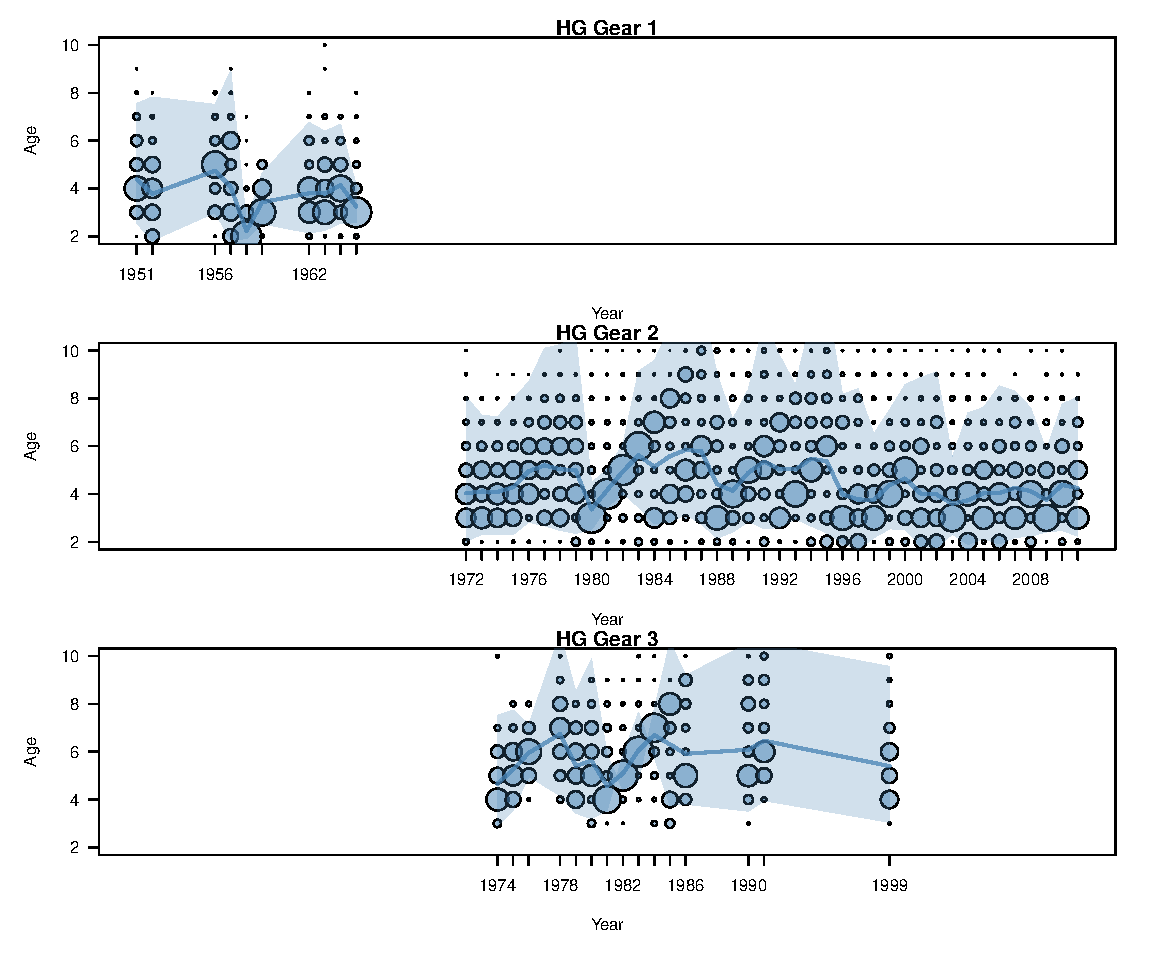
\includegraphics[width=0.85\textwidth]{../Figs/iscam_fig_AgeCompsHG.pdf}\\
	\caption{Bubble plots showing the proportions-at-age versus time for the winter purse seine fishery (top), seine roe fishery (middle) and the gillnet fishery (bottom) in Haida Gwaii.  The area of the circle is proportional to cohort abundance, each column sums to 1, zeros are not shown, and age 10 is a plus group. Also shown is the mean age of the catch (line) and the approximate 95\% distribution of ages (shaded polygon) for each year.}\label{FigAgeCompsHG}
\end{sidewaysfigure}

\begin{sidewaysfigure}[!tbp]
	% Requires \usepackage{graphicx}
	\centering
	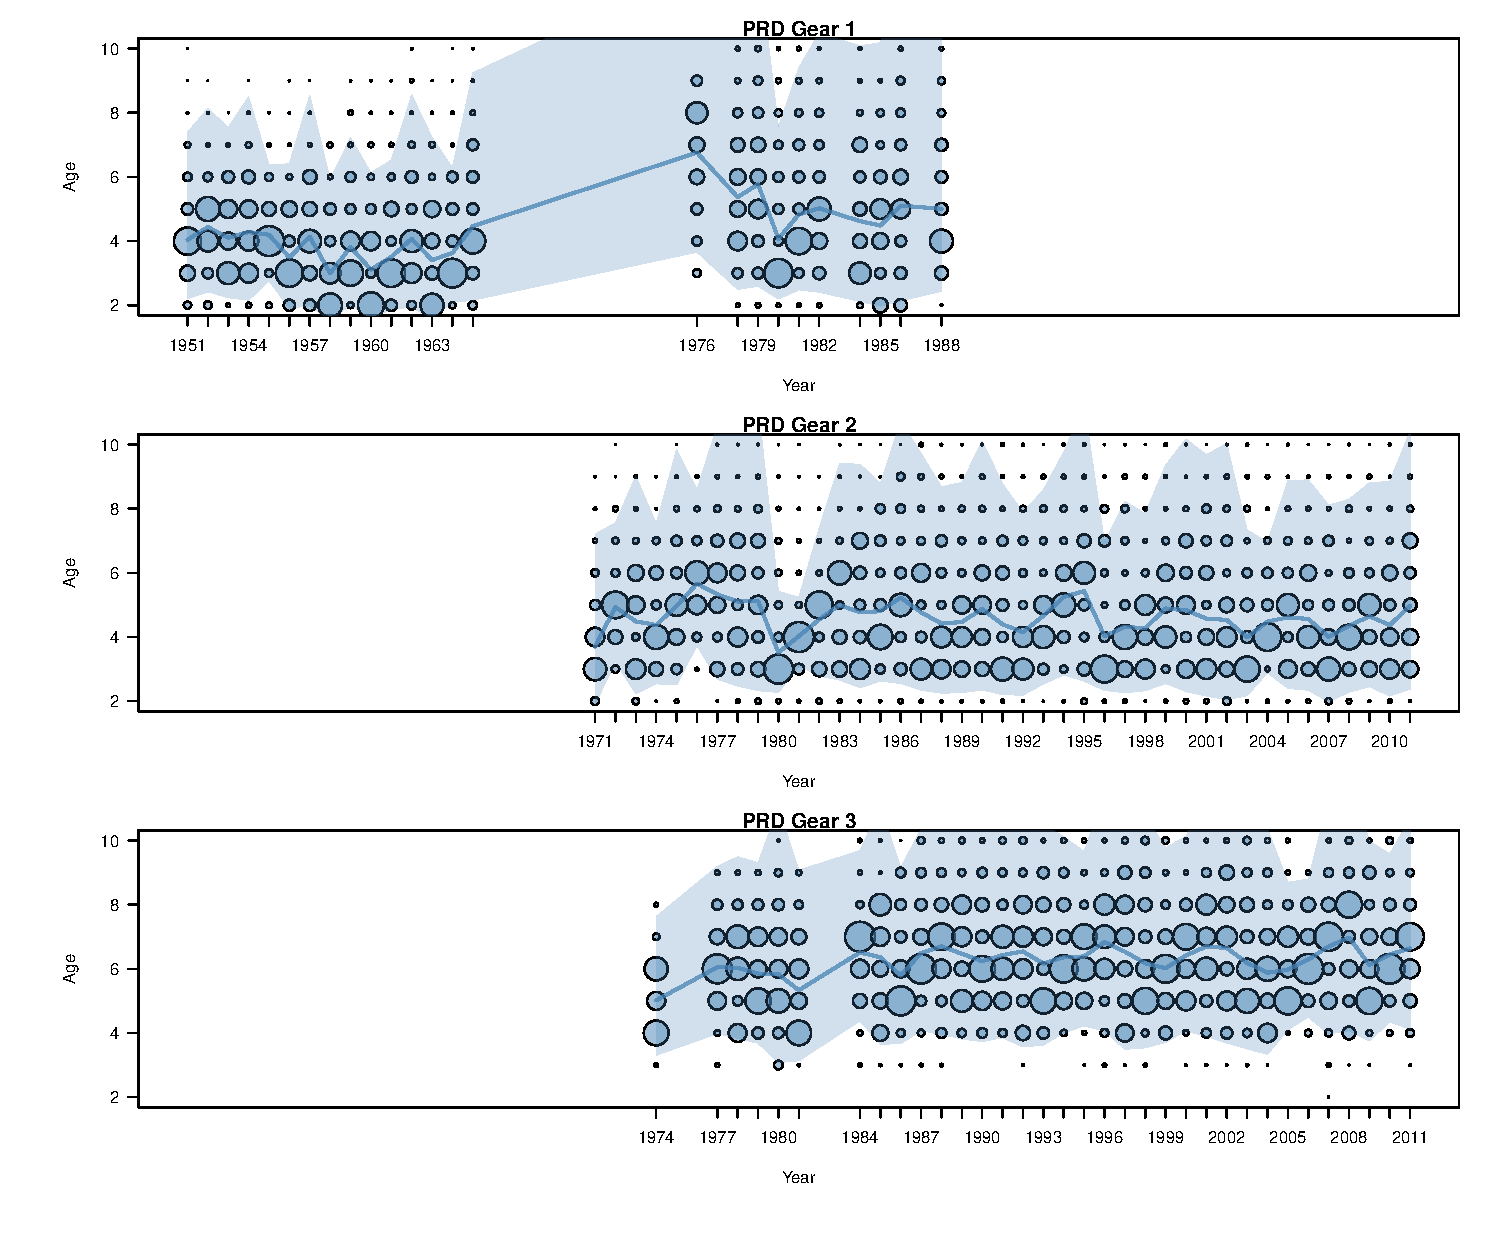
\includegraphics[width=0.85\textwidth]{../Figs/iscam_fig_AgeCompsPRD.pdf}\\
	\caption{Bubble plots showing the proportions-at-age versus time for the winter purse seine fishery (top), seine roe fishery (middle) and the gillnet fishery (bottom) in Prince Rupert District.  The area of the circle is proportional to cohort abundance, each column sums to 1, zeros are not shown, and age 10 is a plus group. Also shown is the mean age of the catch (line) and the approximate 95\% distribution of ages (shaded polygon) for each year.}\label{FigAgeCompsPRD}
\end{sidewaysfigure}

\begin{sidewaysfigure}[!tbp]
	% Requires \usepackage{graphicx}
	\centering
	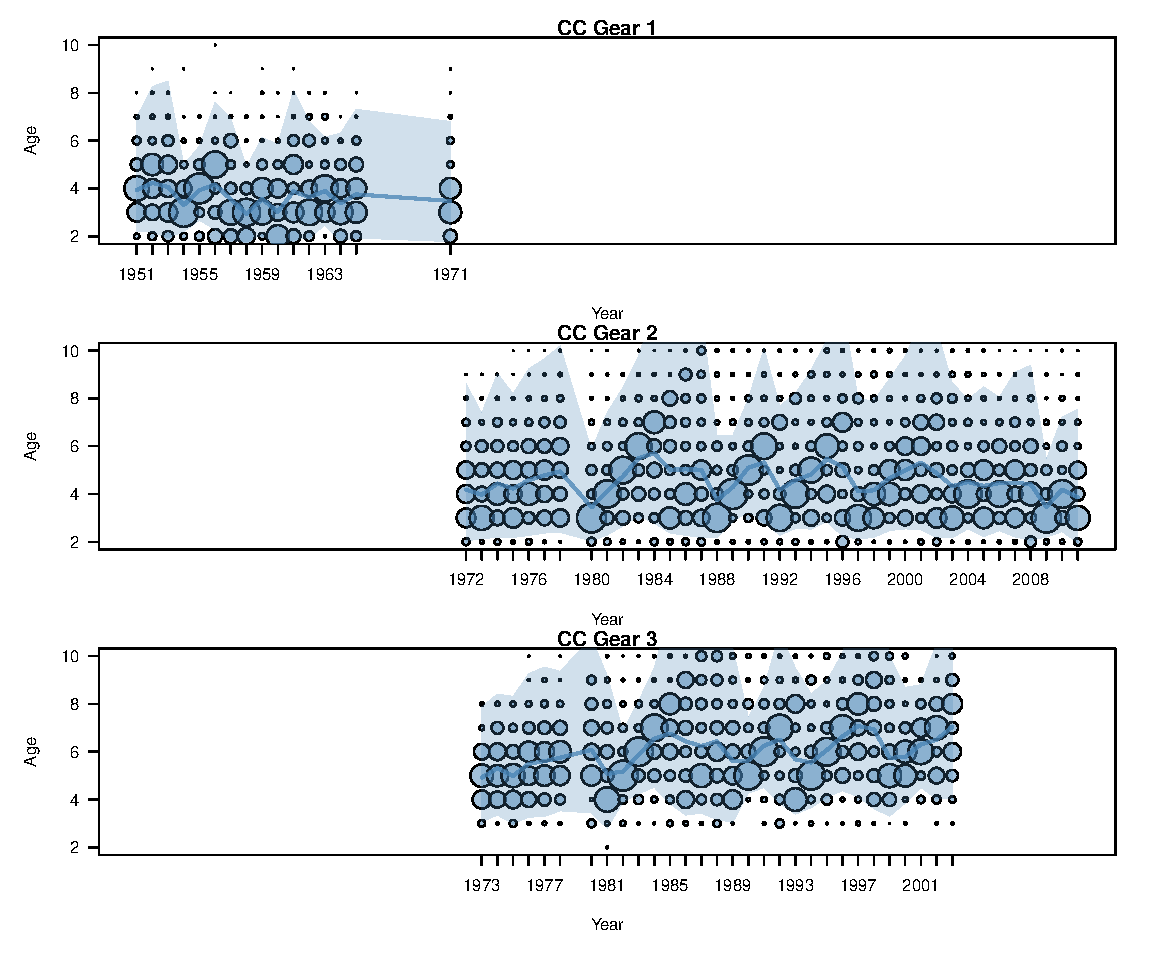
\includegraphics[width=0.85\textwidth]{../Figs/iscam_fig_AgeCompsCC.pdf}\\
	\caption{Bubble plots showing the proportions-at-age versus time for the winter purse seine fishery (top), seine roe fishery (middle) and the gillnet fishery (bottom) in the Central Coast region.  The area of the circle is proportional to cohort abundance, each column sums to 1, zeros are not shown, and age 10 is a plus group. Also shown is the mean age of the catch (line) and the approximate 95\% distribution of ages (shaded polygon) for each year.}\label{FigAgeCompsCC}
\end{sidewaysfigure}

\begin{sidewaysfigure}[!tbp]
	% Requires \usepackage{graphicx}
	\centering
	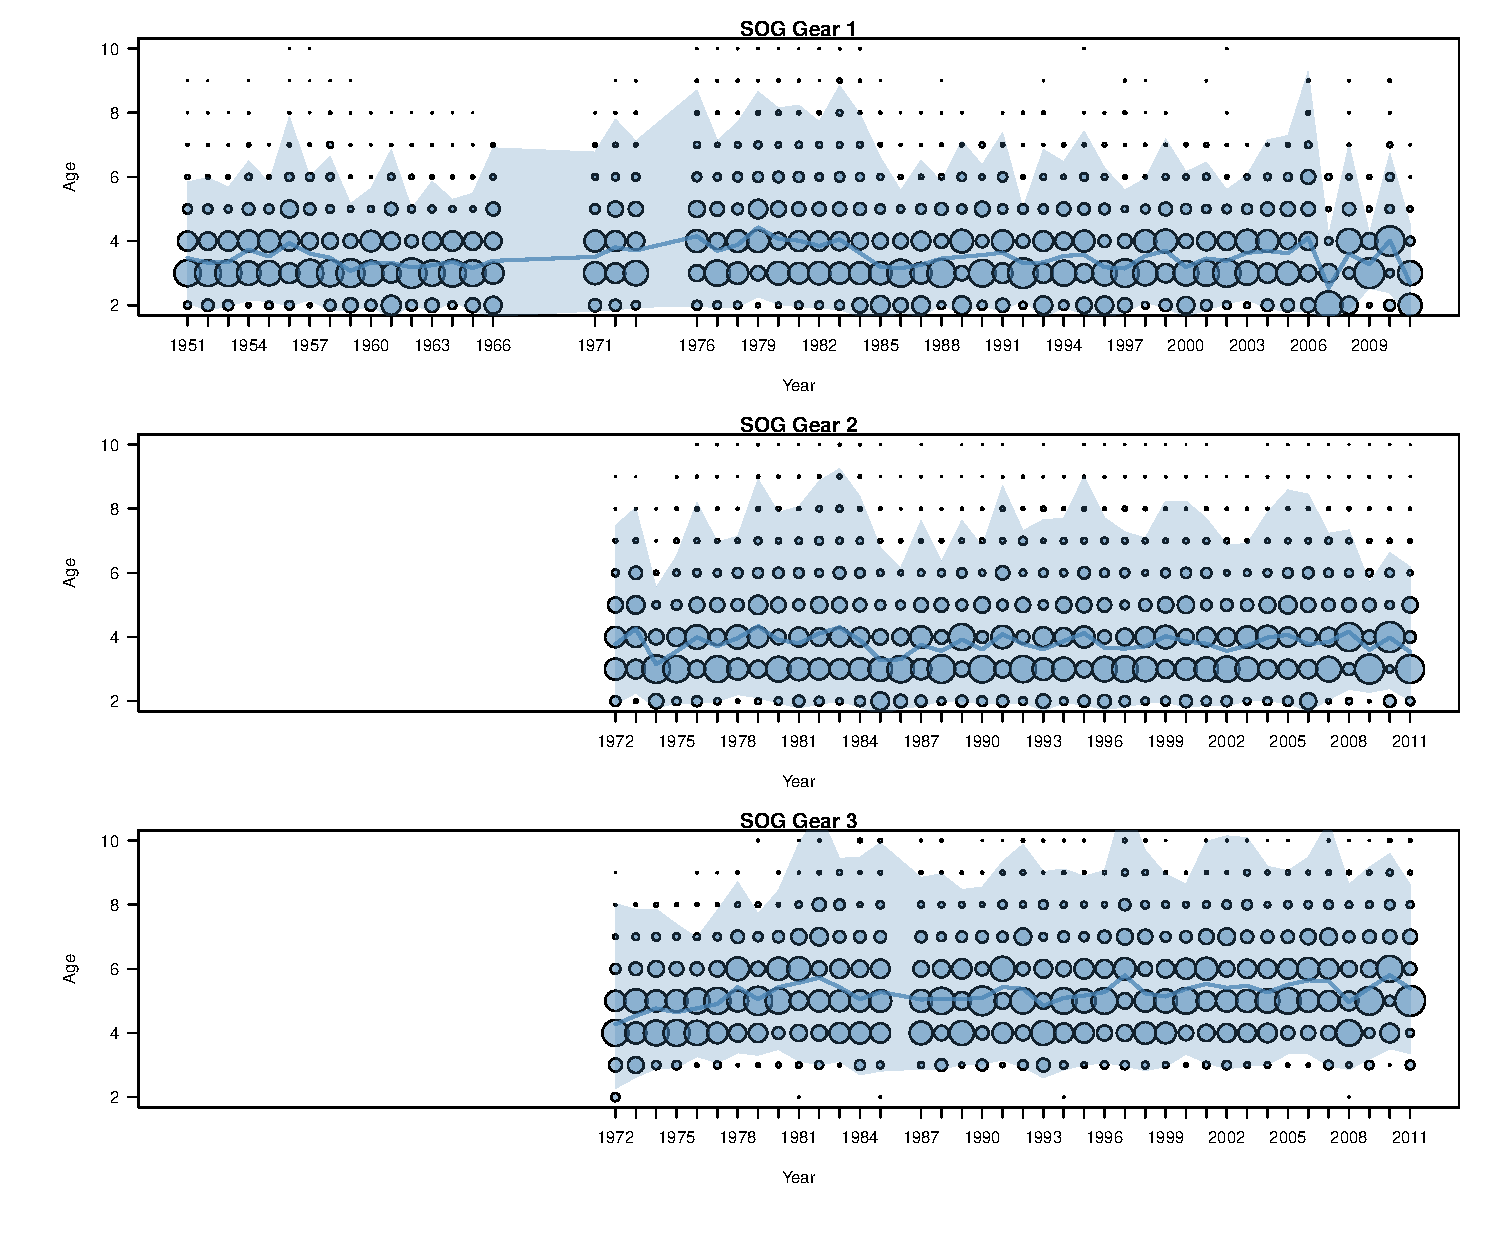
\includegraphics[width=0.85\textwidth]{../Figs/iscam_fig_AgeCompsSOG.pdf}\\
	\caption{Bubble plots showing the proportions-at-age versus time for the winter purse seine fishery (top), seine roe fishery (middle) and the gillnet fishery (bottom) in the Strait of Georgia.  The area of the circle is proportional to cohort abundance, each column sums to 1, zeros are not shown, and age 10 is a plus group. Also shown is the mean age of the catch (line) and the approximate 95\% distribution of ages (shaded polygon) for each year.}\label{FigAgeCompsSOG}
\end{sidewaysfigure}

\begin{sidewaysfigure}[!tbp]
	% Requires \usepackage{graphicx}
	\centering
	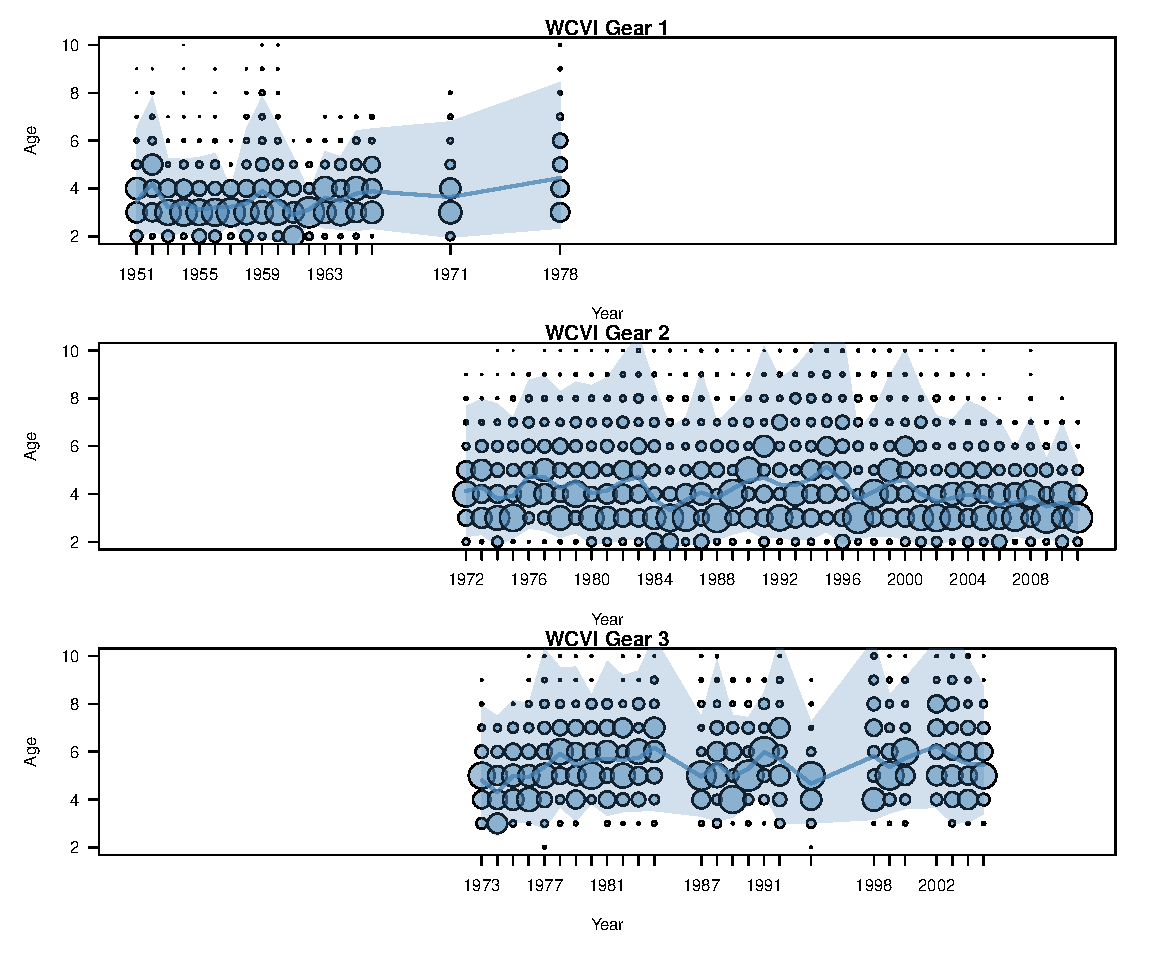
\includegraphics[width=0.85\textwidth]{../Figs/iscam_fig_AgeCompsWCVI.pdf}\\
	\caption{Bubble plots showing the proportions-at-age versus time for the winter purse seine fishery (top), seine roe fishery (middle) and the gillnet fishery (bottom) in the West Coast Vancouver Island region.  The area of the circle is proportional to cohort abundance, each column sums to 1, zeros are not shown, and age 10 is a plus group. Also shown is the mean age of the catch (line) and the approximate 95\% distribution of ages (shaded polygon) for each year.}\label{FigAgeCompsWCVI}
\end{sidewaysfigure}





	\subsubsection{Mean weight-at-age data}

	From the mid-1970s until the present, there has been a measurable decline in weight-at-age for all ages in all major stock areas (Figure \ref{FigMeanWt}). Samples collected during the 2009/10 fishing year indicate weights-at-age that are among the lowest on record. This declining weight-at-age may be attributed to any number of factors, including: fishing effects (i.e., gear selectivity), environmental effects (changes in ocean productivity), or it may even be attributed to changes in sampling protocols (shorter time frame over which samples are collected). Declining weight-at-age has been observed in all five of the major stocks, and despite area closures over the last 10-years, has continued to occur in the QCI and WCVI stocks. Although the direct cause of this decline is still to be investigated, this trend has been observed in B.C. and U.S. waters, from California to Alaska \citep{schweigert2002herring}, and merits further research.	The observed mean weight-at-age data appear to have a few  errors that need to be investigated as well; for example, see the apparently small age-10 fish in 2001 in Figure \ref{FigMeanWt}.

\begin{figure}[!tbp]
	% Requires \usepackage{graphicx}
	\centering
	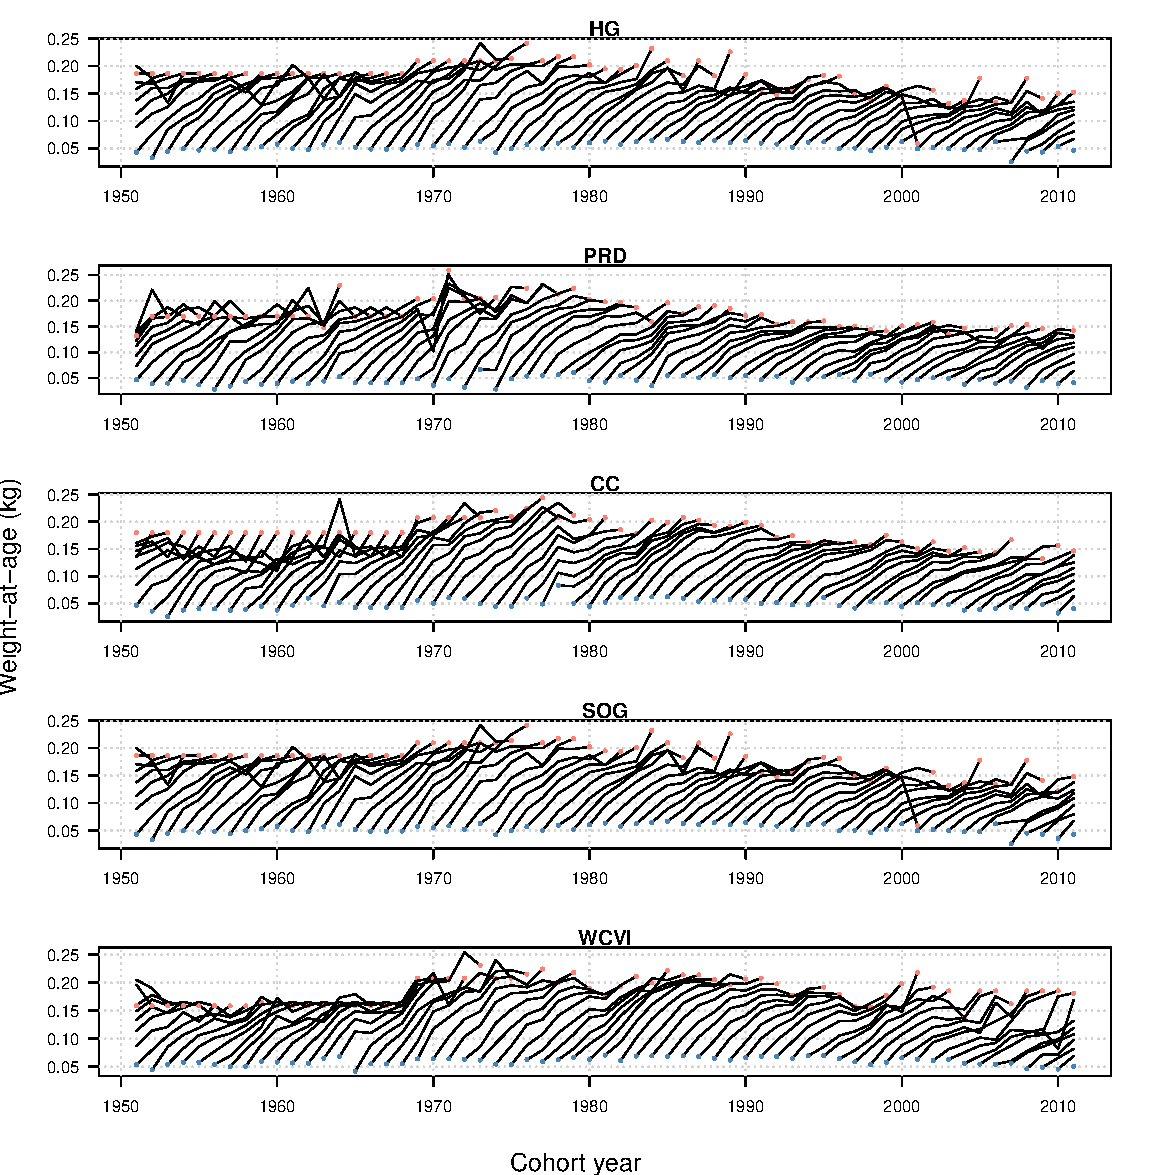
\includegraphics[width=\textwidth]{../Figs/iscam_fig_MeanWt.pdf}\\
	\caption{Empirical mean weight-at-age data by cohort from 1951 to 2011 for ages 2 to 10 in the five major Stock Assessment Regions.}\label{FigMeanWt}
\end{figure}
	

%%%%%%%%%%%%%%%%%%%%%%%%%%%%%%%%%%%%%%%%%%%%%%%%%%%%%%%%%%%%%%%%%%%%%
%%%%%%%%%%%%%%%%%%%%%%%%%%%%%%%%%%%%%%%%%%%%%%%%%%%%%%%%%%%%%%%%%%%%%
%%%%%%%%%%%%%%%%%%%%%%%%%%%%%%%%%%%%%%%%%%%%%%%%%%%%%%%%%%%%%%%%%%%%%	
	\subsection{Analytical methods}

	For the 2011 BC herring assessment, \iscam was used to conduct the stock assessment for each of the five major Stock Assessment Regions (SAR) and two minor assessment areas (Area 2W and Area 27).  The technical details of this model can be found in Appendix \ref{appiSCAM}.
		
	\subsection{Retrospective analysis}
	A retrospective analysis was conducted for each of the major and minor SARs.  The retrospective analysis successively removes the last 10-years of data and examines changes in estimates of terminal spawning biomass.  The results are then plotted on a single panel to compare how estimates of spawning biomass change as successive years of data are omitted from the analysis.
	
	\subsection{Abundance and recruitment forecasts}
	The abundance forecast for the upcoming fishing season, also referred to as pre-fishery biomass, is defined as the predicted biomass of age-4 fish and older plus the number of age-3 fish recruiting in year $T+1$.  The abundance estimates are based on the median values from the sampled posterior distribution.  Age-3 recruits are based on poor, average, and good recruitment scenarios; see next paragraph for definitions of poor, average and good.
	
	The recruitment forecasts are based on the surviving number of age-3 fish at the start of the fishing season times the average weight-at-age 3 in the last 5 years. The definitions of poor, average, and good recruitment are as follows: \textbf{Poor} is the average recruitment from the 0-33 percentile, \textbf{Average} is the average recruitment from the 33-66 percentile, and \textbf{Good} is the average recruitment from the 66-100 percentile.  Note that all cohorts from 1951 to 2011  were included in the calculation of recruitment quantiles.
	
	\subsection{Catch advice}
Catch advice is based on the application of the harvest control rule (HCR). The herring HCR has three components:
\begin{enumerate}
\item Reference points (LRP, USR, and cuttoffs)
\item Harvest rate
\item Decision rules
\end{enumerate}

For each of the five major stocks, the limit reference point (LRP) is the cuttoff value, which is defined here as 0.25\bo\, and the	Upper Stock Reference (USR) is defined as the 1.05*LRP (0.25\bo\ + 0.2*0.25\bo = LRP + 0.05LRP). \textbf{For clarification, references to \bo\ throughout this document refer to the mature spawning stock biomass.} The default harvest rate if the stock is at or above USR is 0.2, and declines linearly to 0 when the stock is at or below the LRP (a default harvest rate of 0.1 is used for the minor stock areas).  The decision rule for the major stock areas operates as follows:

\begin{itemize}
	\item If the forecast run is less than the LRP (cuttoff) then the area is closed to all commercial harvest  (i.e., stock is deemed to be in the critical zone).
	
	\item If the forecast run is greater than the LRP and less than the USR (i.e., cautious zone), then total allowable catch is based on a reduced harvest rate that would deplete the stock to the LRP level.
	
	\item If the forecast run is greater than USR, then the total allowable catch is set at 20\% of the forecast run.
\end{itemize}



	


\part{Effects of reduced minimum-size limits on yield, spawning biomass, and wastage.}
\setcounter{chapter}{2}

\textbf{Objective:} investigate the short-term and long-term consequences of adopting a smaller (26 inch or 66 cm) size limit on halibut spawning biomass, exploitable biomass, yield, and wastage.




%% -End of main body of the document------------------------------------

  %% -References
\clearpage
%input "Refs.bib"
%\bibliographystyle{plainnat}
\addcontentsline{toc}{section}{References}
\bibliographystyle{apalike}
\bibliography{$HOME/Documents/ARTICLES/Articles-1}


%% Appendices
\appendix

\addtocounter{section}{0}
\renewcommand{\thetable}{A-\arabic{table}}
\setcounter{table}{0}
\setcounter{chapter}{1}
%!TEX root = /Users/stevenmartell/Documents/iSCAM-project/fba/Halibut/WRITEUP/Halibut.tex


\section{Input files for the Simulation Model} \label{appen:dataFiles}

In this appendix, the input data, parameter controls and initial parameter values for the Halibut simulation model are given.  Electronic copies of these files are available from a code repository hosted at: \url{http://code.google.com/p/iscam-project/source/browse/}.  The source code is also available from the same repository under the Halibut branch.  A history of the code development can be viewed here: \url{http://code.google.com/p/iscam-project/source/list?name=halibut}.


The following is the data file where, the \# symbol to the left of any number denotes comment lines to document the data file.


\tiny
\begin{alltt}
\input{../DATA/Halibut_2sex_develop.dat}
\end{alltt}
\normalsize


The following text is the control file for the halibut simulation model
\tiny
\begin{alltt}
\input{../DATA/Halibut_2sex_develop.ctl}
\end{alltt}
\normalsize


\tiny
\begin{alltt}
\input{../DATA/Halibut_2sex_develop.pin}
\end{alltt}
\normalsize

\setcounter{chapter}{2}
%!TEX root = /Users/stevenmartell/Documents/iSCAM-project/fba/Halibut/WRITEUP/Halibut.tex

\section{Model Description} % (fold)
\label{sec:model_description}

The following detailed documentation is a description of the simulation model used to generate model output in this report.  The description is broken down into three subsections: 1) simulation model input, 2) state dynamics, and 3) model outputs.  A series of tables along with a detailed written description is used to document the model.  The tables of equations are meant to represent the logical progression of using input data to initialize the population model, simulating dynamical responses to alternative policies and deriving model outputs.

To summarize the following subsections that describe the model in detail, the following pseudocode represents the general order of operations (implemented as specific functions within the computer code).

\noindent\underline{Pseudocode:}
\begin{enumerate}
	\item Read simulation model inputs, (biological data, fishery data and model parameters).
	\item Initialize model parameters (initial age-structure, annual recruitment, etc).
	\item Calculate length-based selectivities for each gear type for each sex.
	\item Partition fishing mortality to each fishing sector.
	\item Calculate age-specific total mortality rate for each year where the probability of capture and discard is a function of selectivity and size limits.
	\item Calculate numbers-at-age each year based on annual values of $Z$.
	\item Compute model outputs and performance measures.
\end{enumerate}

The underlying model design is and age-structured population model with an annual time step.  The population model has two periods: (1) a historical period in which the population model is initialized with numbers-at-age in the first year, and annual recruitments for each year upto the present, and (2) a projection period where the numbers-at-age are simulated 15 years into the future under alternative scenarios and harvest policy options.  Information for the initialization of the population model is based on the most recent stock assessment for Pacific Halibut (Hare 2012 citation).  At each time step in the model, total age/sex-specific mortality rates are computed as a sum of natural and fishing mortalities from each of the directed and non-directed fisheries.

Each fishing gear within the 

% -----------------------------------------------------------------------------
\subsection{Simulation model input} % (fold)
\label{sub:simulation_model_input}

List of model input:
\begin{enumerate}
	\item Historical catch data, or fishing mortality rates.
	\item Annual recruitment from 1996 to present.
	\item Initial numbers-at-age by sex.
	\item Stock parameters ($B_0$,$h$,$M$)
	\item Selectivity parameters (length-based selectivity)
	\item Size limit, target harvest rate, \& other policy related parameters (e.g., SUFD).
\end{enumerate}

\begin{table}[ht]
	\caption{List of symbols, units and description of variables for the simulation model.}
	\label{tab:ListOfSymbols}
	\begin{center}
	\begin{tabular}{ccl}
		\hline
		Symbol & Units & Description \\
		\hline
		$h$	& - & index for sex\\
		$i$	& - & index for year\\
		$j$	& - & index for age\\
		$k$	& - & index for gear\\
		\multicolumn{3}{l}{\underline{Input Parameters}}\\
		$R_0$	& millions	& unfished recruitment\\
		$h$		& -			& steepness of the stock-recruitment relationship\\
		$M_h$	& yr$^{-1}$	& instantaneous natural mortality rate by sex \\
		$\bar{R}$ & millions & average recruitment\\
		$\ddot{R}$ & millions & initial recruitment\\
		$\omega_i$ & - & annual recruitment deviation in year i\\
		$\ddot{\omega_j}$ & - & initial recruitment deviation for age j\\
		\hline
	\end{tabular}
	\end{center}
\end{table}

% subsection simulation_model_input (end)
% -----------------------------------------------------------------------------
\subsection{Analytical description} % (fold)
\label{sub:analytical_description}

% 1) Initial states
% 2) Selectivities and joint probablity for fishing mortality & discard mortality.
% 3) Calculating fishing mortality rates from 1994-present conditioned on catch.
In the more recent stock assessment models, the age/sex/size composition of the commercial landings are estimated externally to the model.  These data are not readily available to be used in this analysis.  The sex composition of the commercial catch was approximated by applying the same fishing mortality rate to each of the sexes, where the fishing mortality rate was approximated by the historical total landings divided by the simulated exploitable biomass (both sexes combined).  This differs substantially from the methods used to apportion commercial catch to each sex \cite[see][for details]{clark2004method}.


% 4) Calculate sex- age-specifc total mortality rates

% subsection analytical_description (end)
% -----------------------------------------------------------------------------
\subsection{Model outputs} % (fold)
\label{sub:model_outputs}

% subsection model_outputs (end)


% section model_description (end)


\end{document}
